%\documentclass[twocolumn]{aastex63}
\documentclass[apj,iop]{emulateapj}
%\documentstyle[11pt,aas_macros]{article}
\usepackage{graphicx}
%\usepackage{subcaption}
\usepackage{subfigure}
\usepackage{amssymb,amsmath}
\usepackage{natbib}
\usepackage{gensymb}
%\bibliographystyle{aasjournal.bst}
\bibliographystyle{apj}
%\bibliographystyle{plainnat}
\usepackage{epsfig}
\usepackage[flushleft]{threeparttable}
\setcitestyle{notesep={; }} %changes "," to ";" in Lang (2014, hereafter L14)
%\renewcommand{\thefootnote}{\fnsymbol{footnote}}
%\graphicspath{{./allfigures/}}
\usepackage{tabularx}

\begin{document}

%\title{Optical-faint, Far-infrared-bright {\textit{\textbf Herschel}} Sources
%in the CANDELS Fields: Ultra-Luminous Infrared Galaxies at \boldmath$z>1$ and
%the Effect of Source Blending
%\footnotemark[$\star$]}\footnotetext[$\star$]{Herschel is an ESA space 
%observatory with science instruments provided by European-led Principal
%Investigator consortia and with important participation from NASA.}

\title{Paper I. 
}
\author{Marat Musin \altaffilmark{1,2}, Jiasheng Huang \altaffilmark{1},
Haojing Yan \altaffilmark{2}, 
}

\altaffiltext{1}{Chinese Academy of Sciences South America Center for Astronomy
(CASSACA), National Astronomical Observatories, Chinese Academy of
Sciences, Beijing 100012, China}
\altaffiltext{2}{Department of Physics \& Astronomy, University of Missouri,
Columbia, MO 65211, USA}



\begin{abstract}
Context: What can be the use of this catalog?

Aims: We present a catalog of XX galactic and 14 million extragalactic sources with photometric redshifts in Stripe 82 with deep data from SDSS and WISE. 

Methods: In order to get consistent photometry, optical sources are convolved to the same PSF for the WISE data we perform "template fitting" - technique that uses high resolution optical sources as a prior to obtain total flux of the low resolution near-IR sources.

Results: T-PHOT code that does "template fitting" uses high resolution and low resolution PSFs to extract robust flux even when source have little flux in near-IR and would not appear in WISE catalog or when sources are blended. Morphological star-galaxy separation is performed and then for each source four photometric redshifts are  calculated using SED fitting code (with and without near-IR bands) EAZY and machine learning code ANNz (using two different training set). Available data allows to retrieve photometric redshift up to z$\sim$0.8  with the average scatter XX.

Conclusions: Our final catalog with photometry and appropriate errors, CLASS\_STAR indices, photometric redshift and cross-matched spectroscopic data within Stripe 82 is publicly available at XXX.XXX.com

\end{abstract}

\keywords{
 infrared: galaxies --- submillimeter: galaxies ---  galaxies: starburst ---
 methods: data analysis
}

\section{Introduction}

\subsection{Lilly-Madau formalism}

\subsection{SED fitting as a standard technique of mass and redshift estimation}
SED fitting is now a standard technique of deriving stellar mass and photometric redshifts for a large set of galaxies. In this method multi-band photometry for a given galaxy is fitted to a series of a templates predicted by a certain stellar population synthesis (SPS) model. The best-fit template gives the parameters of the galaxy, including its redshift and mass.
Historically, SPS models were using restframe optical photometry. One caveat is the degeneracy between the dust extinction and age of the stellar population, as both make the color of galaxy red, i.e. galaxy can be red because it is intrinsically red with no young massive star and ongoing star-formation, or it can be very dusty, or it can be metal-rich and metals effectively absorb light in the bluer bands. Solution to this is to implement restframe near-IR where light suffers much less extinction (comparing to restframe UV and optical) and thus the degeneracy can be broken.
We aim to build the largest sample of galaxies with optical and near-IR photometry over a large sky area. The natural choice for us then is to use optical Sloan Digital Sky Survey (SDSS) and IR all-sky data from Wide-Field Infrared Survey Explorer (WISE).

\subsection{problems associated with construction of the catalog}
Blending, poor spatial resolution in IR
our method – template fitting

\subsection{Goal of this paper}

In this paper we present our technique for construction a catalog of galaxies with reliable SED data in optical and near-IR in Stripe 82 field. We discuss data selection, sources identification in different bands and problems associated with it.

\section{Data Description}


\subsection{SDSS and Stripe 82}

The imaging component of the SDSS, which was done in five broad bands ($u' g' r' i' z'$), has covered 14,555 deg$^2$. In most area, the SDSS only scanned for one pass at an exposure time of 53.9 seconds per band, and thus is rather shallow (for example, the $r'$-band 5 $\sigma$ limiting magnitude is 22.2~mag). For this reason, in most cases the SDSS can only probe the normal galaxy population up to $z\approx 0.4$. However, the Stripe 82 region, which is a long stripe along the equator that spans $20^h < RA < 4^h$ and $-1.26^o < Dec < 1.26^o$, totalling in $\approx$300 deg$^2$ is the exception. It was repeatedly scanned ($\sim$70-90 times, depending on RA) for calibration purpose during the survey \citep{Adelman-McCarthy2007}, and thus the combined scans can reach much better sensitivities.

A number of teams have created deep Stripe 82 stacks and made them available to public. The first such stacks were produced by \citet[][]{Annis2014} based on the data obtained up to December 2005 (20-35 runs), which achieved 1-2 magnitude deeper limits than the single-pass SDSS images. Several other teams \citep[e.g.,][]{2009AJ....138..305J, 2014MNRAS.440.1296H} produced different stacks using different procedures to optimize the image qualities.

\citet[][hereafter J14]{Jiang2014} released a new version of stacks using only the images that were taken under the best weather conditions. These stacks are $\sim0.2$~mag deeper than those produced by \citet[][]{Annis2014}, reaching 5$\sigma$ limits of 23.9, 25.1, 24.6, 24.1, 22.8~mag in $u' g' r' i' z'$, respectively, and also have better PSF characteristics. We adopt these stacks in our work.

\subsection{Structure of SDSS Stripe 82 files}

We use description from J14 to present the structure of optical data. An SDSS run (strip) consists of six parallel scanlines, identified by camera columns (Figure~\ref{fig:sdss}). The scanlines are 13.5 arcmin wide, with gaps of roughly the same width, so two interleaving strips make a stripe that consists of total 12 scanlines (columns). 

%\begin{figure}[!ht]
%\includegraphics[width=6in]{THE ONE THAT HAOJING SENT ME}
%\caption{sample text}
%\label{fig:sdss_s82}
%\end{figure}

The size of each co-added SDSS image is 2854 x 2048 pixels, or roughly 18.8' x 13.5' (RA x Dec), with a pixel size of $0.396^{''}$ and an average full width at half maximum (FWHM) of $\sim1.5^{''}$ in u-band, $\sim1.3^{''}$ in g-band, and $\sim1^{''}$ in r-, i-, and z-bands. In total there are 401 SDSS images in each column and overall $12 \cdot 401 \cdot 5 = 24,060$ SDSS images in all 5 bands. Each SDSS image has a corresponding $weight.fits$ image, that records relative weights at individual pixels.

\subsection{WISE and unWISE}

%WISE \citet{Wright2010} is a near-IR space observatory that was launched in December 2009 and mapped the entire sky with sensitivity far better than that of its predecessors, IRAS \citet{Neugebauer1984} and DIRBE \citet{Silverberg1993}. With a 0.4 m telescope on board always pointing at 90 degrees solar elongation, WISE made successful scans of the entire sky in four bands, namely W1 ($3.4 \mu m$), W2 ($4.6 \mu m$), w3 ($12 \mu m$) and w4 ($22 \mu m$). Its bands W1 and W2 are far more sensitive than w3 and w4 ( ..... mJy respectively) and can be used to extend SED of the galaxies to the near-IR, break age/dust degeneracy and account for numerous low-mass stars when calculating the stellar mass. It is natural that IR data have much worse pixel scale comparing to optical, so matching data from different data sets has always been an issue. We address this problem in the next section when talking about template fitting, but prior to that we shall have another look at WISE.

%WISE has the best resolution among near-IR telescopes (e.g. IRAS \citet{Neugebauer1984} and DIRBE \citet{Silverberg1993}) that have covered all Stripe 82. Its bands W1 (3.4 $\mu m$, 54 $\mu Jy$) and W2 (4.6 $\mu m$, 71 $\mu Jy$) are far more sensitive than  w3 (12 $\mu m$, 730 $\mu Jy$) and w4 (22 $\mu m$, 5000 $\mu Jy$) 

% and can be used to extend SED of the galaxies to the near-IR, break age/dust degeneracy and account for numerous low-mass stars when calculating the stellar mass.


WISE \citep{Wright2010} is a near-to-mid IR space telescope launched in 2009 and has performed an all-sky imaging survey in four bands at 3.4, 4.6, 12, and 22~$\mu$m (denoted as W1, W2, W3, and W4, respectively). 
During its original mission phase from 2010 January 7 to 2010 August 6 (the “4-band Cryogenic” phase), WISE surveyed the entire sky 1.2 times in all four bands simultaneously until the solid hydrogen coolant in the outer cryogen tank was depleted. It then entered the “3-band Cryogenic” phase for the next 54 days, during which time it mapped an additional 30\% of the sky in W1, W2 and W3. When the coolant in the inner tank was also depleted by 2010 September, only W1 and W2 are operational. The NEOWISE project took over the mission on 2010 October 1 and brought it into the four-month “Post-Cryo” phase to survey the sky in these two bands for near-earth objects until 2011 February 1 \citep[see][]{2014LPI....45.2724M}. The telescope was then put into hibernation for the next 35 months as the funding stopped. The extended NEOWISE project reactivated it in 2013 December to continue the two-band observations (“NEOWISE Reactivation”) through today.

The WISE team made three data releases separately for the 4-band Cryogenic, the 3-band Cryogenic and the NEOWISE Post-Cryo phases in 2012 March, 2012 June and 2013 May, respectively. To take the advantage of these repeated observations, the WISE team also made the ``AllWISE Data Release’’ in 2013 November by combining all the WISE data available till then \citep[see][for details]{2013wise.rept....1C}. The included image products,
%By the end of survey operations in February 2011 it has completed three mission phases, namely WISE Cryogenic Survey, WISE 3-band Survey and NEOWISE Post-Cryo Survey \citep{2011ApJ...731...53M}.
% Complete all-sky coverage in two epochs was achieved after three mission phases, namely WISE Cryogenic Survey (120$\%$ of the sky is covered), WISE 3-band Survey (W4 band excluded, 30$\%$ of the sky is covered) and NEOWISE Post-Cryo Survey (only bands W1 and W2 were used, 70$\%$ of the sky is covered). 
%Three separate mission phases, namely WISE Cryogenic Survey, WISE 3-band Survey and NEOWISE Post-Cryo Survey allowed WISE to perform an all-sky coverage in two epochs.
%The nominal 5~$\sigma$ limits in four bands are 0.08, 0.11, 1.0, and 6.0~mJy, respectively \citep[see][for details]{Wright2010}.
%W1, W2, W3, W4 (3.4, 4.6, 12, and 22 $\mu m$, respectively). The 5$\sigma$ limits are better than 0.08, 0.11, 1, and 6 mJy for these four bands (see Wright et al. (2010) for more details).
%The AllWISE Data Release 1 was announced 2013 Nov 13, and includes data taken during the first three mission phases: the 4-band primary mission, the 3-band phase (W1, W2, W3), and the NEOWISE post-cryo phase (imaging only in W1 and W2). The data products in the AllWISE Release include coadded matched-filtered images known as the ``Atlas Images''. Atlas Images are intentionally convolved by the point-spread functions (PSFs) for better detection of isolated sources. 
%This operation reduced the resolution and created the blending problem in the crowded fields. \citet[][; hereafter D14]{Lang2014e} restored original pixel scale and preserved the spatial resolution of original images. His set of co-adds achieves 6" PSF full-width half maximum (FWHM) in W1, W2 and W3 bands and 12" in W4.
%The WISE team made the AllWISE Data Release 1 in 2013 November. The image products included in this release, 
known as the ``Atlas Images'' reach the nominal 5~$\sigma$ limits of 0.054, 0.071, 0.73, and 5.0~mJy in the four bands, respectively. 

To optimize the detection of isolated sources, the WISE team has been using a special treatment when combining images, namely, the single-exposure images are convolved with the individual point spread function (PSF) during the stacking process. However, this operation has the drawback that it reduces the spatial resolution of the final stacks, which is not desirable in many applications. To deal with this problem, \citet[][hereafter L14]{Lang2014e} reprocessed all the WISE images independently without the PSF convolutions, and produced the stacks that preserve the original WISE spatial resolutions. These image products of L14,  dubbed as the ``unWISE'' images, have the PSF full-width at half maximum (FWHM) values of $6^{''}$ in W1, W2 and W3 and $12^{''}$ in W4. Sensitivity of bands W3 and W4 is $\sim$10 times worse than that of bands W1 and W2 and is not sufficient so that at least 10$\%$ of the optical sources have secure W3 and W4 fluxes. We use  unWISE W1 and W2 images for this work.

\subsection{Structure of unWISE files - once again maybe I need to omit it in the paper}

The unWISE coadds are on the same tile centers as the WISE tiles with 18,240 images per band, 1.56 x 1.56 degrees each. The tiles are named by their RA, Dec center: tile "0591p530" is at RA = 59.1, Dec = +53.0 degrees; i.e., the first four digits of the tile name is $int(RA \cdot 10)$, then "p" for +Dec and "m" for -Dec, then three digits of $int(abs(Dec)\cdot 10)$. For each tile and band W1-w4, several images are produced, we shall list only the ones that we make use of:

-- unwise-0000p000-W1-img-m.fits - "Masked" image, 2048 x 2048 pixels, TAN projected at 2.75"/pixel. Background-subtracted, in units of "Vega nanomaggies" per pixel: $mag = -2.5 \cdot (log_{10}(flux) - 9)$. This is the science image, the word "masked" means that some pixels have no unmasked pixels and no measurement at all: pixel value 0 and infinite uncertainty.

-- unwise-0000p000-W1-std-m.fits - Sample standard deviation (scatter) of the individual-exposure pixels  contributing to this coadd pixel.\\

Three unWISE images centered at the same RA cover the whole width of Stripe 82 in Dec ($-1.26^o$ to $+1.26^o$). We shall call three such unWISE images a frame. There may be up to 72 SDSS images within one frame.

\subsection{Spectroscopic sample}
Spectroscopic redshifts are used to perform star/galaxy separation and calibrate photometric redshift estimation: determine a set of templates and photometric offsets for the template-fitting code and train machine learning algorithms. We shall call such full sample of sources a star/galaxy catalog and a subset with only sources classified as galaxies or QSOs with $z_{spec}>0$ as spectroscopic catalog. Originally, we constructed our training set using spectroscopic data from the SDSS DR14 (\citet{Bolton2012a}). Spectroscopic redshifts and classification into galaxies, stars and QSOs for the SDSS DR14 catalog are calculated using principal component analysis (PCA). The software $\tt idlspec2d$ is used to perform, at each potential redshift, a least-squares fit to each spectrum, using a fairly general set of models, for galaxies, for stars, for cataclysmic variables, and for quasars. The best fit model and redshift is chosen and assigned for the object.

Their spectroscopic sample consists of a wide variety of galaxies, stars and QSO with no cuts on color, although it is rather limited in terms of redshift (\citet{Strauss2002}. Stripe 82 data are 1-2 mag deeper than single-pass images and therefore potentially has a lot of sources at higher redshifts. We decided to extend our training set by cross-matching galaxies in our photometric catalog with spectroscopic measurements of other, publicly available surveys, such as 6dF, WiggleZ, DEEP2, VVDS and VIPERS.

In Tab.\ref{tab:table1} we list auxiliary catalogs with selection criteria, median redshifts for galaxies and QSO and total number of sources that were added to our training set. For each source, we use published redshift quality flag to select trustworthy sources, but also add stars when possible (which sometimes have special flag or assigned with negative redshift).

We cross-matched the galaxies from the star/galaxy set with our photometric catalog using 2'' as maximum separation in RA and Dec and this resulted in 268,587 sources - galaxies (59\%), stars (29\%), QSOs (11\%) and not classified objects (1\%).

\begin{table*}[t]
  \begin{center}
    \caption{Catalogs with spectroscopic redshifts.}
    \begin{threeparttable}
    \begin{tabular}{|p{1.6cm}|p{3cm}|p{3.5cm}|p{2.9cm}|p{2.5cm}|p{2cm}|}
      \toprule % <-- Toprule here
      \textbf{Survey Name} & \textbf{Selection criteria} & \textbf{References} &\textbf{Number of sources in the star/galaxy\tnote{1} (spectroscopic\tnote{2} ) set}  &  \textbf{Median redshift of the spectroscopic set} & \textbf{Comments}\\
            \hline
      SDSS DR14 &  zErr $<$ 0.1 and zWarning = 0 & \citet{Bolton2012a} & 225,076 (115,359) & 0.316 &  \\
      6dF & Q = 3, 4, 6 & \citet{Jones2004}, \citet{Jones2009} &  375 (328) & 0.054 & no zErr\\
      WiggleZ & Qop = 3, 4, 5 & \citet[][]{Drinkwater2010}, \citet[][]{Parkinson2012a} &  10,674 (9,555) &0.550 &\\
      DEEP2 & ZQUALITY = 3, 4 and zErr $<$ 0.01 or CLASS = STAR & \citet[][]{Davis2003c}, \citet[][]{Newman2013} & 15,730 (11,683) &  0.957 &\\
      VVDS & 1 $<$ ZFLAGS $<$ 20 & \citet[][]{LeFevre2013}, \citet[][]{Garilli2008} & 10,137 (8,383) &  0.602 & no zErr\\
      VIPERS & 2 $<$ zflg $<$5 and classFlag=1 and zspec $>$ 0 & \citet{Scodeggio2018}, \citet{Guzzo2014} & 6,595 (5,460) & 0.690 & $\sigma_z$ = 0.00054$\cdot$ (1 + z)  \tnote{3}\\
       Full sample &   &  &  268,587 (150,767) & 0.409 &\\
             \hline 
    \end{tabular}
\begin{tablenotes}    
    \item[$^1$] Includes stars, galaxies, QSOs and unidentified sources with secure redshift. The sample is used for the star-galaxy separation.
    \item[$^2$] Includes galaxies and QSO and is used for EAZY and ANNz testing.
    \item[$^3$] No $z_{spec}$ errors are provided, these values are given in the paper.
     \end{tablenotes}
    \end{threeparttable}
      \label{tab:table1}
  \end{center}
\end{table*}


\section{Overview of Methods for Analysis}

The most critical factor in SED fitting is consistent photometry in the involved bands, i.e., the photometry should include the same fraction of light across all bands so that the colors are defined in a consistent manner. This is challenging in our case because the spatial resolutions of WISE are at least $6\times$ worse than that of the SDSS. For this reason, the objects detected in WISE often suffer blending. Even for relatively isolated WISE sources, the photometric apertures appropriate for the (low resolution) WISE images cannot guarantee the same fraction of light being included as what is done in the (high resolution) SDSS images. Such a systematic offset, which is different for every galaxy, severely skews the SED fitting. 

To best address this problem, we opt to use the $\tt T-PHOT$ software \citep[][]{Merlin2015}, which recently emerged as a robust and flexible tool to perform ``template fitting''. The basic idea is to use a high-resolution image (here an image from the SDSS) as the prior to build the morphological template of the source under question, convolve this template with the PSF of the low-resolution image (here the corresponding image from the unWISE), and fit this degraded template to the low-resolution image to obtain the total flux that is within the aperture as defined by the high-resolution image. In this way, we get reliable color information (i.e., flux ratio) in the most consistent manner. 
%It is important to note that high-resolution source does not have to be point-like - its morphological features will be preserved and fitted to the low-resolution source. This implies the biggest assumption for this technique - that morphology of the source is wavelength-independent. While generally it is not true, we anticipate that this will not create any significant bias. Firstly, because most of the galaxies have small angular sizes and such variation is negligible (galaxy at z=0.7 that is 40 kpc in diameter has an angular size of only 6 pixels), and secondly, because we chose SDSS r-band (6202.46 $\AA$), as a high-resolution image - there should not be much morphological difference between r-band and W1 or W2 bands.

While $\tt T-PHOT$ is much more user-friendly as compared to its predecessors (i.e. TFIT \citet[][]{Laidler2007}), running this software is still non-trivial. It not only requires careful tuning of parameters but also several tedious preparatory steps with both the high- and the low-resolution images. Here we detail our procedures.
	

\subsection{Initial preparation of unWISE and SDSS images} 

%T-PHOT input files must satisfy certain requirements: the high- and the low-resolution images should have the same type of projection, reference coordinate and orientation as written in their FITS headers. We verify that SDSS and WISE images indeed have the same tangential projection and orientation ($CD1\_2 = 0, CD2\_1 = 0$). Meanwhile each WISE frame covers $\approx 3.95\, deg^{2}$ and there may be up to 72 SDSS images that cover the same area, so we use coordinates of the center of WISE images (CRVAL1 and CRVAL2) as the anchor values and run SWarp [Bertin et al., 2002] to change reference pixels in all SDSS images. The reference pixel (CRPIX1 and CRPIX2) for SDSS images can now be outside of the image itself to as far as 0.7 deg.

%T-PHOT input files must satisfy certain requirements: the low-resolution background-subtracted image must have the same orientation as the high-resolution image (i.e. no rotation allowed), and the origin of one pixel must coincide. Reference pixels (CRPIX) in all SDSS images within one unWISE footprint were changed using SWarp \citep{Bertin2002} to match the world coordinate values (CRVAL) for a given unWISE image. $\approx15\%$ of the SDSS images have more than one unWISE image within its footprint. Such images were duplicated and assigned with different reference pixels, thus increasing the number of SDSS files from  4812 to 5556 images per band.

T-PHOT requires that the low- and the high-resolution images have the same orientation and the same World Coordinate System (WCS) reference position, the latter of which is defined by the FITS keywords (CRVAL1, CRVAL2). %We chose to change the SDSS images to match the unWISE images, because an unWISE image is always oriented to North-up and East-left and encompasses multiple SDSS footprints. 
It also requires that their pixel scale ratio must be an integer. To meet these prerequisites, we carried out the following procedures utilizing the {\tt SWarp} software \citep[][]{Bertin2002}, which can subsample or bin an image to any pixel scale and then re-project to an arbitrary orientation at any tangential point.

%The change to the SDSS images was done by using the SWarp software \citep[][]{Bertin2002}. The reference pixel (CRPIX1 and CRPIX2) for the SDSS images can now be outside of the image itself to as far as 0.7 deg.
We first rescaled the unWISE images from 2.750\arcsec/pix to 2.772\arcsec/pix. As the scale of an SDSS image is 0.396\arcsec/pix, this makes the ratio of their pixel scales an integer ($2.772/0.396=7$). We kept the same orientation, which is always North-up and East-left, and the same reference position for each unWISE image. This process was done for both the W1 and the W2 unWISE images, which are always aligned.

For a given SDSS image, we oriented it to North-up and East-left, and re-projected it at the tangential point as defined by the reference position of the unWISE images that it lies within. In other words, the FITS keywords (CRVAL1, CRVAL2) of the re-projected SDSS image are the same as those of the unWISE images. As an unWISE image covers much larger area and thus encompasses multiple SDSS footprints, the tangential projection point of a reprojected SDSS image is often outside of its coverage. In the extreme cases, it can be as far as 0.7\degree outside of the image itself.

About 30\% of the SDSS images' footprints lie across two adjacent unWISE fields, and therefore need to be treated separately. If an SDSS image has more than 60 arcmin$^2$ belonging to adjacent unWISE fields, such image is duplicated, and each copy is reprocessed with respect to the appropriate unWISE field as described above. This increases the number of SDSS images from 4,812 to 5,556 per band. All SDSS images in col02 and col11 have $\sim$2.9' overlap with unWISE images centered at Dec=-1.7 and Dec=1.5 respectively. Processing of such small region requires construction of $\sim$930 PSFs per band and 2,000 hours of CPU time and is unviable. This excludes 11.34 deg$^2$ from the total area for which catalog is constructed.

We note that the above procedures were done for both the science images and the standard deviation (for the unWISE) or the weight (for the SDSS) images. After the subsampling and re-projection, the standard deviation or the weight value per pixel no longer preserves the absolute scale. In other words, the value of a given pixel on an unWISE (SDSS) reprojected standard deviation (weight) image no longer reflects the true standard deviation (weight) on that pixel. Fortunately, this does not affect the performance of $\tt T-PHOT$, as it only uses these values in a relative sense (i.e., the absolute scale does not matter). 

***
{\it describe unWISE cutouts for each SDSS image?}
***

We also note that one special treatment needs to be done for the saturated pixels in the unWISE standard deviation images. They are all assigned with zero values in the unWISE release, which is invalid for $\tt T-PHOT$. We therefore use the $\tt IRAF/imcalc$ task to set such values to “9999” before reprocessing.
    
%Some SDSS images lay at the interface between two adjacent WISE images. Such SDSS images ($\approx15\%$) were duplicated and each copy was assigned with different reference pixels, thus increasing the number of SDSS images from 4,812 to 5,556 per band.

%The WISE images were rescaled from 2.75 ''/pix to 2.772 ''/pix using SWarp. The pixel scale ratio of WISE images and SDSS images is thus an integer: $2.772/0.396 = 7$.

%Center pixels of saturated sources in the WISE standard deviation images have zero values and that is an invalid input for T-PHOT. $\tt IRAF/imcalc$ task was used to detect such pixels and change its value to ``9999''.

%There are SDSS files that lie in the overlapping region of two adjacent unWISE images. In such a case we duplicate SDSS image and run SWarp twice, assigning new SDSS image reference coordinates from each of the adjacent unWISE images. This operation reduced the blind zone but increased the number of SDSS files from  4812 to 5556 images per band.

% * construction of the PSF and kernels
\subsection{Input SDSS source catalog} 
J14 produced object catalogs from their stacked images using $\tt SExtractor$ \citep[][]{Bertin1996}. While it is tempting to use them directly as the input source catalogs for $\tt T-PHOT$ on the unWISE images, several caveats prevented us from taking this approach. For example, these catalogs are not cleaned of duplicated sources from the overlapped areas between adjacent images; they are not matched among the bands and thus have different number of sources for each band; the object detection threshold was set too high and many faint objects were excluded; bright and saturated objects have clusters of false detection; etc. For these reasons, we constructed our own input source catalogs.

\subsubsection{Rationale}
%Due to the great depth, roughly 24.6 AB and $\approx1''$ PSF FWHM r-band was chosen as a reference band. Centroids, morphology, and other non-amplitude parameters of the detected sources are then fixed to the values from this reference band. Sensitivity, FWHM and local background varies in SDSS from band to band, so neither aperture, nor Kron flexible elliptical aperture \citep{Kron1980} can produce consistent colors in 5 optical bands, which is crucial for the subsequent SED fitting.

%To remedy this problem, all individual images in $g'r'i'z'$ bands are convolved to the PSF of the corresponding image in the band with the worst PSF FWHM, namely u-band. For the price of losing some sources due to blending in the reference band, matched to the u-band, we extract more robust fluxes. Matching one images in one band to the PSF of the image in the different band requires knowledge of the kernel - a PSF matching function between two images. The PSF of SDSS images varies in RA (corresponds to image rows), due to atmospheric fluctuations and, as a result, different seeing. It also varied in DEC (corresponds to columns), due to camera optics and different airmass. Thus there is no universal PSF and individual PSF must be built for each SDSS image. Construction of the 27,780 PSFs in Stripe 82 (5,556 per band) is the most time-consuming part of the project.
In addition to providing input source information to $\tt T-PHOT$, our SDSS catalog also provides optical SEDs for all the detected sources. For the latter, it is critical that the colors of a given source are measured consistently across all five bands, or in other words, the photometric aperture of a source must include the same fraction of total light in any given band. To achieve this goal, we took the standard approach by performing ``PSF-matching’’ of the SDSS images. For a given SDSS field, we first matched the size of the PSF in g, r, i, and z-bands ($\sim 1.0$—1.3\arcsec) to that of u-band, which always has the largest PSF ($\sim 1.5$\arcsec; see J14). We then ran matched-aperture photometry using r-band as the reference band, which detects more sources than any other band.

The PSF-matching step was the most tedious part of the process, which required a lot of human intervention. To derive the convolving kernels between two images, we first must obtain the PSFs of both images. As the SDSS PSF varies from image to image, we had to construct it for each image individually. In total, we built 27,780 SDSS PSFs (5,556 per band).

\subsubsection{PSF construction and PSF-matching}
An empirical PSF is best derived by combining a large number of bright, isolated point sources (also known as the ``PSF stars’’) distributed over the entire image, given that PSF is constant across the image. The most robust method to derive a PSF is to run the $\tt IRAF$ task “psf” interactively on a list of candidate PSF stars and to retain only the best ones in the construction. Given the huge number of images involved, however, this was not practical. After  extensive tests, we settled on an approach that would result in reliable PSF stars, which would then allow us to run the “psf” task non-interactively in most cases.

   The key in the PSF star selection is to determine whether an object is a point source of high image quality. We first removed the objects that are saturated or too faint. The magnitude cuts are typically $\sim xx$ and $\sim xx$ mag at the bright and the faint ends, respectively. We then used the stellarity identifier produced by $\tt SExtractor$, ``CLASS\_STAR’’, to select the potential point sources. The output value of this parameter ranges from 0 (most likely non-stellar) to 1 (most likely stellar), and we rejected the objects that have CLASS\_STAR~$< 0.85$. The survived candidates were further refined by comparing their ``core’’ magnitudes and the total magnitudes. The smaller the difference between the two means the more compact the object is. The size of the aperture depends on the particular band, and is $\sim 3.56$\arcsec\, in general. We adopted the criterion of $<0.xx$ mag for this difference in this refinement. Finally, we only retained the stellar objects that are not close to the image edge ($>xx$ pixels to the boundary) and do not have a neighbor within XX\arcsec.
   %. Our approach was to compare the ``core’’ magnitude and the total magnitude. The smaller the difference between the two means the more compact the object is. We used SExtractor MAG\_APER and MAG\_BEST to quantify the core and the total magnitudes, respectively. The size of the aperture depends on the particular band, but in general is $\approx$ 3.56$''$. The second selection involved magnitude cuts (saturated and faint sources were removed) and the use of the stellar classification technique. The later was estimated using SExtractor which uses a neural network as a classifier to assign the values from 0 to 1 to the stellarity parameter CLASS$\_$STAR, respectively. Sources with CLASS$\_$STAR$\sim$1 appear to be point-like, so objects with CLASS$\_$STAR$<$0.85 were rejected. As the last step, we only left the source in the final sample if it is not close to the edge of the image and does not have another nearby source within XX$''$. 

%Finally, each SDSS image has 20 to 160 point-like sources that contribute to the PSF model. Lower value appears in a few images when there are not enough bright point sources (mostly in the less sensitive u-band), while the cut in the maximum number of the point sources was performed in order to have stable performance of the {\tt IRAF/psf} task. \textit{I know it sounds ugly, but I don't want to write the IRAF sometimes  crashes when you supply more than 160 stars.} Visual inspection is given to all constructed PSFs. If it shows some features, such as elongation, gradient of the background due to the nearby (within up to several arcmin) bright source, or faint non-detected blended source in the vicinity of the main profile, then manual selection of the point sources and reconstruction of the PSF is performed. {\tt IRAF/seepsf} is used to take the PSF, computed by the {\tt IRAF/psf} and build a 21x21 pixel output FITS image, consisting of the sum of the analytic function and the residual. All PSF images are subsequently normalized to the unity total counts using 

The retained point sources were then supplied to the $\tt IRAF/psf$ task for PSF construction. Typically, each SDSS image had more than 20 point sources in the end to build its PSF. Lower value appeared in only a few images, most of which are in the less sensitive u-band. On the other hand, there are plenty of images that have hundreds of qualified point sources, and using all of them would actually make the PSF construction exceedingly time-consuming. Therefore, we applied an upper limit of 160 point sources per image when running $\tt IRAF/psf$. 

***
Parameters, Moffat function
***

The output from this task was then convereted by using $\tt IRAF/seepsf$ to the format that can be further used. At this point, we visually examined all the resulted PSFs. If a PSF showed some undesirable features indicative of contaminations (for examples, elongation, gradient in the wing, neighbors not identified previously), we would manually reject the problematic point sources and rebuild the PSF.  Finally, all the PSF images were normalized to the total count of unity using {\tt wcstools/sumpix} \citep{Mink1998b} and {\tt IRAF/imarith} tasks. 

Before the PSF matching could be carried out, we would need the transferring kernal between the two PSFs under question. This was done by suppling the PSFs to {\tt IRAF/lucy} that uses the algorithm developed by \citet{Richardson1972} and \citet{Lucy1974}. Finally, the PSF-matchinng to the u-band was performed by {\tt IRAF/psfmatch} that used the g’r’i’z’ images and the relevant kernels as the inputs. For the sake of simplicity, we shall refer to these u-band PSF-matched images as the ``g2u’’, ``r2u’’, ``i2u’’, and ``z2u’’ images, respectively. 

A subtle problem with PSF matching is that the convolution introduces extra correlation among nearby pixels, which artificially suppresses the noise. In other words, the noise of the PSF-matched images would be underestimated if it were measured by the pixel-to-pixel background fluctuation. We will return to this point in the next section.

\subsubsection{Optical catalog construction}

%Catalogs are produced running {\tt SExtractor} in the dual mode, where r-band matched to u-band ("r matched to u" for short) is used for detection and all five bands (u-band, g matched to u, r matched to u, i matched to u, z matched to u) are consequently used for photometry. Catalogs in each image are then matched by their ID. Original weight images were used for both detection and photometry. As a result, even spurious detections have SNR$>$5 and real objects have non-realistic associated magnitude errors, which affect the choice of proper templates for SED fitting. This effect is clearly seen on the left part of Figure~\ref{fig:magerr_corr_example} - magnitude errors are plotted against AB magnitudes for all sources from a random image in the g-band. Blue points represent sources from the original g-band image, red points - from the "g matched to u" image. Individual ratio of the magnitude errors per source and than the mean ratio for all the sources was calculated. Right panel of Figure\ref{fig:magerr_corr_example} shows such mean ratio for all 5,556 images in the g-band. Black vertical line denotes the ideal ratio of "1". Magnitude errors in the "g matched to u" images are considerably underestimated throughout the whole Stripe 82 as compared to the magnitude errors in the original g-band images and this situation persists in all 5 bands. We mitigate such problem by running {\tt SExtractor} in the dual mode again, with r matched to u image as a detection and original $g'r'i'z'$ SDSS images for photometry. Then for each source, e.g. in g-band, with photometry determined in the "g matched to u", photometric error is assigned from the original g-band image. We emphasize that photometry and photometric error belong to the same problem since the same "r matched to u" image is used for detection.

The catalogs were produced by running SExtractor in the dual-image mode, where the r2u images were set as the detection images and the photometry was run in turn on the u, g2u, r2u, i2u, and z2u images. 

*** You’re missing a lot of details here!!!  You should provide these:

- What is the filter?

- What is the detection threshold?

- What is the number of connecting pixels (DETECT\_MINAREA)?

- What flavors of magnitude are derived?

***

The image weighting scheme was set to ``MAP\_WEIGHT’’, and we used the original weight maps from J14. Strictly speaking, these weight maps no longer reflect the pixel-to-pixel weights because the science images have been convolved. Nonetheless, this does not significantly impact the source detection because the general trend of the weight is still preserved (e.g., it is unlikely that the convolution would transform a low-weight pixel into a high-weight one). 

   However, as the correlation of pixels due to the PSF matching is not taken into account by these weight maps, the photometric errors reported in our {\tt ISExtractor} runs are underestimated (except in u-band because the u-band images were not convolved). This is demonstrated in the left panel of Figure 1, where we show the MAGERR\_AUTO vs. MAG\_AUTO diagram for a randomly chosen g-band image. The blue and the red points represent the photometry using the original g-band image and the g2u image, respectively. The same weight image was used in both cases. Clearly, the red points are below the blue ones, or in other words, the photometric errors on the PSF-matched image are significantly underestimated. 

%SNR$>$5 cut in the "r matched to u" band removes spurious sources and leaves XX,XXX,XXX sources with optical photometry.

%We mitigate such problem by correcting magnitude errors for bands $g'r'i'z'$. For each image {\tt SExtractor} was ran again in the dual mode with r matched to u as a detection and original $g'r'i'z'$ SDSS images for photometry. As illustrated on the left panel Figure~\ref{fig:magerr_corr_example}, two catalogs for each image (original image and matched to u-band) are stacked and the mean ratio of the original SNR to matched SNR for all sources is calculated. All magnitude errors in a matched image are then multiplied by this ratio that is denoted as the coefficient K to correct for the underestimated magnitude errors (Figure~\ref{fig:magerr_corr_example}, right). Coefficients K range from 1.1 to 2.5 in four bands, with the mean values XX, YY, ZZ and ZZ for bands $g'r'i'z'$, respectively. All 5556 coefficients for the g-band color-coded by the column number are shown  on Figure~\ref{fig:all_band_corr}. In addition to statistical errors there are systematic error that are accounted by adding in quadrature a value of 0.04 magnitudes. Each source in each band is thus assigned with the error magnitude that was calculated using the following equation:
%$$ magerr\_corrected = \sqrt{0.04^{2}+(\dfrac{1.0857}{SNR}\cdot K)^{2}} $$ SNR is FLUX$\_$ISO $ \//$ FLUXERR$\_$ISO and K is correction coefficient. SNR $>$5 cut was applied and the catalog at this stage consists of 26,585,000 sources. 

\begin{figure}
\begin{minipage}{\columnwidth}
\includegraphics[width=\columnwidth,height=0.28\textheight]{figures/figure_magerr_corr_gband_example_uncorr.png}
%\includegraphics[width=0.5\linewidth]{figures/figure_hist_mean_gband.png}
\caption{Magnitude error vs. absolute g-band magnitude for one SDSS image. Mmagnitude errors in the g2u image(red) are underestimated as compared to the original SDSS g-band magnitude errors (blue).}
%Right panel: histogram of the mean ratio of the original magnitude errors over magnitude errors in the "g matched to u" image for each of 5,556 images. Black vertical line denotes the mean ratio of 1.}
%\hfill
\label{fig:magerr_corr_example}
\end{minipage}
\end{figure}

%For that reason $g' r' i' z'$ bands were convolved to the PSF of the one with the worst FWHM, i.e., u-band. In such a case the size variation in different bands will be attributed to the intrinsic difference in morphology at different wavelength. For the price of loosing some sources due to blending, more robust optical colors will be extracted. Matching is performed with $\tt IRAF/psfmatch$ task that requires supplying the image with the corresponding kernel - PSF matching function. Building a kernel requires  knowledge of the PSFs of the input image and a matched image. Construction of 27, 780 PSFs in Stripe 82 (5, 556 per band) is the most time-consuming part of the project.
%One of the widely-used ways to construct PSF is by using PSFEx software [Bertin, 2011]. We tested it with T-PHOT and found that the quality of residual images is not satisfactory, so we decided to use more conservative algorithm in which IRAF/psf task creates a PSF function based on a set of selected point-like sources (so called PSF stars). Usually that strategy involves consecutive run of IRAF/find, IRAF/phot, IRAF/pstselect and IRAF/psf tasks that find stars, determine its magnitude, select the ones that do not have any morphological features and finally construct a PSF function. This algorithm, though very reliable, is also not ideal - in each image there are $\approx 10\%$ of sources that do not satisfy the criteria of PSF stars (are elongated, blended or have noisy background) and have to be rejected in the manual regime (selection in interactive mode). This is extremely time-consuming and inefficient given the total number of images in 5 bands. We decide to use a variation of this method to create PSF functions in a more automatic fashion.

%We run SExtractor on each SDSS image and only mark sources from the output catalog as a point-like, if their ”stellarity” index (determined by a CLASS STAR parameter) is close to 1, sources are bright, but not saturated, they do not lay within 2$\cdot$ PSF radius to the edge of the FITS image, and have all their flux contained within some small aperture. The later was calculated as the difference ”MAG diff” between MAG APER that returns all flux within some fixed aperture and MAG BEST that returns MAG AUTO value in the absence of contamination from the nearby sources and MAG ISOCOR otherwise. Exact parameters depend on the band and also were adjusted during test runs so that each SDSS image has no less than 20 PSF stars (stars were sorted by their magnitude, from bright to dim), with the maximum number of PSF stars limited to 160 (larger values significantly slow down IRAF).

\subsection{Kernels for T-PHOT}

%Now the optical part of the catalog is compiled and we start to work with near-IR data to get consistent flux . Template fitting requires a kernel - PSF matching function between the high resolution and the low resolution images. We used the same strategy as outlined in the section 3.2.2 and also positions of the PSF sources in r-band to construct PSF in ``r matched to u'' band which is used as a prior for the unWISE W1 and W2 low resolution images. Due to broader profiles after PSF matching, some PSF sources now have contamination from the neighbor sources. Such PSFs are reconstructed using  {\tt IRAF/psf} in the interactive mode.

%Though generally space telescopes have stable PSF due to the absence of the atmosphere variations and PSF models averaged over the focal plane can be used (such approach is used in e.g. D14), we constructed individual PSF for every unWISE image in the Stripe 82 footprint. The reason behind it is that WISE Atlas Images are constructed by co-adding many single-exposure images. Because the number and relative orientation of single-exposures differ significantly between Atlas Tiles, and because the single-exposure PSFs vary with focal plane location, the PSF will be different for every Atlas Image and will vary with position on any given Atlas Image. \textit{mostly took it from allsky supplementary materials, might need rephrasing}
%http://wise2.ipac.caltech.edu/docs/release/allsky/expsup/sec4_4c.html

%There are 240 unWISE images within Stripe 82 footprint per band. 480 PSFs are constructed in a similar way to the SDSS PSFs with only one change, namely all point-like sources were selected in interactive mode using  {\tt IRAF/psf}. This is done to perform more robust selection of the point sources as 3 PSFs from one unWISE frame are convolved with up to 72 SDSS PSFs and thus its quality is crucial - incorrect PSF profile leads to wrong flux estimation and also creates characteristic positive and negative ring-shaped patterns in the residuals.

Running {\tt T-PHOT} requires the convolution kernel between the Hi-res and the Lo-res PSFs, which in our case are the PSFs of the SDSS ``r matched to u'' images and the unWISE W1 and W2 images, respectively. While in theory the PSF of a ``r matched to u'' image should be the same as that of the u-band image, in reality the matching is never exact. Therefore, we could not use the u-band PSFs but had to construct the PSFs of the ``r matched to u'' images to optimize the performance of {\tt T-PHOT}.  We already had a list of point sources when constructing the original r-band PSFs (see \S 3.2.2), which could be used here again. We visually examined them on the ``r matched to u'' images, removed all those that are contaminated by neighbors due to the larger PSF in ``r matched to u'', and used the refined list of point sources to derive the ``r matched to u'' PSFs in the same way as described in \S 3.2.2.

For the unWISE images, we opted to derive their PSFs independently in all tiles instead of using the WISE PSFs as published by the WISE team. While the WISE PSFs were rather stable throughout the mission, they should not be used directly for our purpose because the image stacks are the combination of multiple single-exposure images of varying orientations. As the result, the PSF of a WISE image stack is no longer that of a single exposure, and also changes significantly from tile to tile. 

There are 240 unWISE image tiles within the Stripe 82 footprint, and thus we derived 480 unWISE PSFs (240 each in W1 and W2, respectively) using point sources that were derived in the same way as described in \S 3.2.2. All PSFs were constructed by running {\tt IRAF/psf} interacively.

All the unWISE PSFs were normalized to unity total counts using {\tt IRAF/imarith} and sub-sampled in size by the factor of 7 using {\tt IRAF/imlintran} to match the pixel scale ratio between the unWISE and the SDSS images (see \S 3.1). %IRAF/lucy is used to convolve normalized ``r matched to u'' PSFs with normalized and sub-sampled unWISE PSFs to create individual kernels.
Finally, we used {\tt IRAF/lucy} to generate the individual convolution kernels between the ``r matched to u'' images and the unWISE images. In total there are 11,112 kernels: 5,556 as a result of convolving ``r matched to u'' to W1 band and 5,556 - convolving ``r matched to u'' to W2 band.

\subsection{Running T-PHOT}
%T-PHOT is a software designed to perform a precision photometry on a low-resolution images using information provided by a high-resolution images of the same field as a prior. Running T-PHOT on such a large portion of the sky with individual kernel for every pair of high- and low-resolution images is a key feature of our project.

%Following recommendations from \citet{Merlin2016a} two passes are performed on each pair of images. The first pass performs template fitting using provided kernel and also constructs individual kernels for each source on a given image by applying shifts in high-resolution image reference pixels along X and Y directions. These individual kernels are then used in the second T-PHOT pass. Standard pipelines are used for both passes. Single fitting is applied instead of dividing the low-resolution image on a number of individual cells. The former approach requires large amounts of computational time, but it provides the most accurate flux estimate.

%One of the advantaged of T-PHOT is a large saving of computational time comparing to its forerunners, TFIT or CONVPHOT codes, but it still needs lots of CPU time. T-PHOT has to be run twice (first pass and second pass) in two unWISE bands, W1 and W2 on each of 5556 SDSS images within Stripe 82. One single pass takes $\approx3$ hours CPU time totaling in 66,700 CPU hours for Stripe 82. Computation is performed on the University of Missouri High-Performance Computing (HPC) cluster Lewis to process all images. 

%Once all unWISE images within Stripe 82 footprint in W1 and W2 bands are processed by T-PHOT, output catalogs need to be matched with the optical ones. Matching is performed with STILTS code separately for every image using unique source ID as the matching parameter. Due to poorer sensitivity of the WISE as compared to SDSS, 11,367,420 (39\%) and 12,868,350 (44\%) of sources in bands W1 and W2, respectively were assigned with zero or negative flux. Such sources are kept in the final catalog and are assigned with AB mag = -99 in the corresponding band.
With the r2u source catalogs (\S 3.2.3) and the transformation kernels between the r2u and the unWISE images, we performed {\tt T-PHOT} on each r2u/unWISE pair. This was by far the most computing-intensive step, which was carried out at the Lewis cluster of the High-Performance Computer (HPC) at the University of Missouri.

Following the recommendation of \citet[][]{Merlin2015}, we ran {\tt T-PHOT} for two passes. The first pass performs template fitting “globally” for the Hi-res sources on the Lo-res image at the exact source locations as provided by the input Hi-res source catalog. In the meantime, it also allows the fitting position of each source to shift by a small amount around the prior to find the most optimal position that would result in even better fit than at the prior position. The second pass then uses these refined positions to perform the template fitting again. In all our testing cases, the results from the second pass were significantly improved as compared to those from the first pass, which justified spending extra computing time to finish two passes.

As mentioned in \S 3.1, there are 5,556 SDSS images per band in the Stripe 82. Therefore, there were 5,556 r2u/W1 pairs and the same number of r2u/W2 pairs. Each T-PHOT pass took about 3 hours of computing time at the cluster, and the whole process totaled $\sim 66,700$ hours.

The output {\tt T-PHOT} catalogs in W1 and W2 were merged with the SDSS optical catalogs for the future use. The sensitivity of WISE is not sufficient to detect all the SDSS sources. In total, 11,367,420 (39\%) and 12,868,350 (44\%) r2u sources are not detected in W1 and W2, respectively, and {\tt T-PHOT} resulted in zero or negative fluxes for them. For the sake of completeness, these sources are still kept in the final catalogs and are assigned magnitude of -99.0 in W1 and/or W2.

*****
These are numbers before masking, I am not sure what you mean by "cleaning"
*****


%**matching all 5 bands to the PSF of the u-band**

%When all PSF stars are selected PSF was constructed using standard IRAF/psf. Then we run IRAF/seepsf, a task that takes the input PSF computed by the IRAF/psf task, consisting of the parameters of a 2D analytic function stored in the image header, and computes 21x21 pixel output PSF FITS image consisting of the sum of the analytic function and the residuals. Visual inspection of all PSF images revealed a certain fraction of defect PSFs. The reason for it can be either a blended source within the PSF radius, high background values due to the nearby bright star (within up to several arcmin), or noticeable elongation of the source (may be due to inclusion of a galaxy in our sample or due to intrinsic problems with SDSS image). The fraction of such images varied in different bands but generally was $\approx 4\%$ and for such images we re-run IRAF/psf in interactive mode (manually selecting PSF stars from a pre-selected catalog). All PSF images were normalized to unity total counts using wcstools/sumpix [Mink, 1998] and IRAF/imarith tasks. Several PSFs for all 5 bands and 6 different columns centered at RA=21:56:46 are shown in Figure 3.2. We used IRAF/lucy, a task that uses algorithm developed independently by Lucy [Lucy, 1974] and Richardson [Richardson, 1972], to create kernels for pairs of images in x- and u-bands, where ”x-” stands for g-, r-, i-, or z-band
 
%With kernels in hand it is now possible to run IRAF/psfmatch that convolves input image with the kernel to produce a psf matched output image (Figure 3.3). From when u-band, g-band, r-band etc images mean "SDSS Stripe 82 images stacked by J14 with new CRVAL and new CRPIX values", while g matched u, etc. means images in the g-band matched to the PSF of the u-band image. 
 
% *	catalog construction with SExtractor in dual mode, using r\_matched\_u band for detection
	%SDSS co-adds from J14 already have associated catalogs on the whole Stripe 82 region. We decide not to use it and create our own for several reasons:\\
%	-	J14 catalogs are not matched between the bands, resulting in different number of objects in different bands.\\
%	-	SNR at which the source is rejected is too high and there are a lot of sources that are identified in several bands when we perform our own photometry that were not included in J14 catalog.\\
%	-	Bright and saturated objects are detected as multiple sources, none of which is at the center of such object making correct SED fitting impossible. \\
%	On Figure~\ref{fig:catalog_comp} we show a comparison of the original catalog from J14 (sources within green regions) and our catalog (sources within red regions). In the next 2 subsections we show the strategy for catalog construction with consistent optical colors in all 5 SDSS bands.

%To construct a consistent optical catalog we run SExtractor in the dual mode - the first image is used for detection and astrometry information, while the second is used solely for photometry. We take r mathced u image as detection image and supply consequently all 5 bands to extract photometry of the sources and reject sources with SNR < 5 based on the r matched u flux. R matched u catalogs as well as corresponding segmentation maps also serve as an input to the T-PHOT to derive consistent photometry on near-IR bands. Our parent catalog now consists of 26,585,000 sources. We notice that very few sources were rejected at this stage - objects that appear almost undetectable had FLUX AUTO / FLUXERR AUTO larger than 5 or even 7. 

\subsection{Catalog post-processing}

The merged photometric catalog from the above contains 29,046,660 entries, which would need to go through a few steps before it can be used further. In particular, our major goal is to produce a catalog of galaxies that is suitable for future applications. These steps are detailed below

\subsubsection{Removing duplicate sources}

Adjacent SDSS images have 25'' and 28'' wide overlapping regions in RA and Dec, respectively. Similarly, adjacent unWISE images have 186'' and 180'' wide overlapping regions regions in RA and Dec, respectively. Sources in these regions appear in the catalog more than once and thus the duplications should be removed. 

We performed an internal matching within the catalog, using a matching radius of 1.3\arcsec. We found 1,423,979 duplications, which were subsequently removed from the catalog based on the SNR in the r-band (i.e. the source with the lower SNR is removed, while the source with the higher SNR is kept in the catalog).

\subsubsection{Masking around bright stars}

%Objects that are extremely bright in near-IR present a number of problems to the photometry measurement of the nearby sources because it generates a host of artifacts. These artifacts include halos (low surface brightness emission extending well beyond the PSF), diffraction spikes, stripes of saturated pixels and residual ghosts. These artifacts will compromise the reliability of W1 and W2 photometry performed by TPHOT. To account for such artifacts the natural solution is to mask certain regions based on available catalogs. We used SAO star catalog \citet{Staff1966} and Bright IR Stars Compilation (BIRSC) [R. Tam and C. Xu - IPAC] as a base for the masking catalog. There are around 400 stars in both catalogs within Stripe 82 footprint, but our visual inspection showed that some very bright objects (both stars and galaxies) that severely alters results of TPHOT are still not in this list. We inspected all residual FITS images and added 300 more objects to the list that now consists of 705 objects. Masking area depends on the provided V-band magnitude if exists and visual estimation of the halo size otherwise. Radii for masking are ranging from 50 to 600 arcsec. An example of such source with 100 asec masking radius is shown on Figure 4.8. The overall masked area is 3.866 deg$^2$, which reduces the total sky area of the survey to 288.212 deg$^2$.

Extremely bright objects severely contaminate their vicinities with various artifacts, such as bright halos, stripes of saturated pixels, diffraction spikes, ghost images, etc. As the sources found in such regions are often spurious and their photometry highly unreliable, we opted to remove them entirely from our catalog by masking out such regions. We used the SAO Bright Star Catalog (URL) and the Bright IR Stars Compilation (URL) as the basis of masking. There are around 400 (exact number) stars in both catalogs within Stripe 82, and our visual inspection of the T-PHOT residual images identified 300 (exact number?) additional objects (stars and very bright galaxies). We applied circular masks centered on these 705 sources, where the masking sizes depend on their V-band magnitudes if exist or our visual estimate of the halo sizes otherwise.  The masking radius ranges from 50 to 600 arcsec. We removed the objects detected within the masked regions from our catalog. The maksed area totals 3.866 deg$^2$, which reduces the total sky area of the survey to 288.212 deg$^2$.

%\begin{figure*}[!ht]
%\includegraphics[width=1.0\linewidth]{figures/masking_100asec.png}
%\caption{W1 (left) and W2 (right)T-PHOT residuals of the bright star. Area inside a region with a radius 100 asec (green) is masked. }
%\label{fig:mask}
%\end{figure*}

\subsubsection{Star-Galaxy separation}

%Our catalog now consists of 29,046,660 objects and is contaminated with stars and QSO that should be removed prior to any SED fitting. There are two major ways to classify stars and galaxies in large sky surveys, namely morphological and photometric separation. Morphological approach separates point-like sources (stars and QSO) from extended ones using flux profiles, while photometric separation uses rest-frame optical, near-IR (e.g., AB W1-W2 $\geqslant $ 0.8 cut proposed in \citet{Stern2012} for the AGN detection) or FIR (\citet{Pollo2010}) colors to isolate regions that are mainly populated by stars or QSO. While the former method has a risk of loosing faint compact galaxies that outnumber halo stars at depth r'$>$24 AB, we choose to use it as the primary criterion - photometric separation can hardly be used because star and QSO's loci populate the same space as sources that we classify as galaxies (Figure~\ref{fig:color_color_star_galaxy}), and W1 and W2 bands cannot be used because only 45\% of sources have proper photometry in both near-IR bands. 
% the latter method is not applicable in our case: optical colors cannot be used because star and QSO's loci populate the same space as sources that we classify as galaxies (Figure~\ref{fig:color_color_star_galaxy}), and W1 and W2 bands cannot be used because only 45\% of sources have proper photometry in both near-IR bands. 

Our catalog includes both galaxies and Galactic stars, the latter of which are not the subjects of our study and therefore should be flagged. There are two major ways to separate stars and galaxies, namely, morphological classification and photometric separation. The former distinguishes point-like sources (mostly stars, but also including QSOs) from extended ones, while the latter uses some certain color criteria to separate stars (and QSOs) from galaxies in the color space. We chose to use the morphological method as the primary criterion and the follow up cleaning will be done by the gentle photometric separation using r-i vs. z-w1 color diagram.
%
This was again to utilize the SExtractor stellarity parameter CLASS\_STAR, which we used previously in selecting point sources for the SDSS PSF derivation (see \S 3.2). We ran $\tt SExtractor$ in the dual-image mode again, this time using the r2u images as the detection images and measuring the CLASS\_STAR parameter on the  original g’, r’ and i’ images. An accurate derivation of CLASS\_STAR needs an accurate input of the seeing FWHM value for each image, which we obtained based on the PSFs derived earlier. With the CLASS\_STAR values, we then used the spectroscopic sample of 254,190 sources in Stripe 82 classified by the SDSS team (\citet{Bolton2012a}) to determine the optimal range of CLASS\_STAR. We found that it must simultaneously be less than 0.47, 0.43 and 0.75 in g’, r’ and i’, respectively, to have the lowest fraction of missed galaxies (1.76\%) and contamination from stars and QSO (2.39\%).

%Morphological classification that we decide to apply is based on the SExtractor CLASS\_STAR parameter that is assigned to each object and is bounded within the stellarity index from ''0'' (galaxy) to ''1'' (star). SExtractor uses neural network with the back propagation learning procedure and 10 input parameters: 8 isophotal areas, 1 peak intensity and seeing. Seeing for the given image can be easily estimated as the FWHM of the PSF with $\tt IRAF/imexamine$ and we use the advantage of already constructed PSF for every original (i.e. not matched to the u-band) image in 5 optical bands to find the combination of CLASS\_STAR parameters in different bands that shows the best performance in the star-galaxy separation. We use spectroscopically confirmed sample of 254,190 sources classified by the SDSS team (\citet{Bolton2012a}) to find the optimum: CLASS\_STAR parameters should be simultaneously less than 0.47, 0.43 and 0.75 in bands g'r'i', respectively to have the lowest fraction of missed galaxies (1.76\%) and contamination from stars and QSO (2.39\%).

%Morphological separation of stars/QSOs and galaxies has a risk of misclassification of faint objects that could be compact or distant galaxies. We anticipate that this will not be a major issue: faint galaxies will have isophotes disturbed by the background noise and thus will not appear point-like and distant bright galaxies should not be classified as point sources because average seeing in $g'r'i'$ bands is $\approx1''$ which corresponds to the maximum angular size of 8.464 kpc at z=1.7 which is well below of the diameter of the normal size galaxy.

%The main goal of this project is to create a clean sample of galaxies. After morphological star/galaxy separation was done we determined a locus on the r-i vs z-w1 (?) plane that is mostly populated by spectroscopically confirmed stars that are still present in our sample. We used the color cut XXXXXX to perform the second order star-galaxy separation and it additionally removed XX\% of the stars and XX\% of galaxies from the spectroscopic sample.
After performing star-galaxy separation our catalog contains 14,418,304 galaxies and 13,423,475 point sources (stars and QSOs).

%\begin{figure*}[!ht]
%\includegraphics[width=0.5\linewidth]{figures/color_color_star_galaxy.png}
%\includegraphics[width=0.5\linewidth]{figures/color_color_star_galaxy_2.png}
%\caption{Color-color planes u'g'r' (left) and g'r'i (right) occupied by all sources classified as galaxies (blue) based on morphology are overplotted with stars (green) and QSO (red) that are spectroscopically classified by the SDSS team (\citet{Bolton2012a}). }
%\label{fig:color_color_star_galaxy}
%\end{figure*}

\section{Photometric redshift estimation}

%The distance to an extragalactic source is the quantity that cannot be directly measured, but needs to be inferred before any meaningful physical quantities can be estimated. Distance can be estimated by the stretch of the SED due to the expanding Universe that goes as (1+z), where z is a cosmological redshift. The measured redshift is then related to the proper distance, assuming a cosmological model.

%Redshift is estimated by identifying at least a pair of characteristic features in the SED, such as emission and absorption lines. In addition, there are two broad band features, namely Balmer and Lyman breaks. Balmer break below 4000$\AA$ is caused by the absorption by hydrogen atoms of photons with energy above the Balmer limit at 3,646$\AA$ and also by the combination of the absorption features by ionized metals in the stellar atmospheres. Lyman break below 1,216$\AA$ is explained by the absorption of photons below the Lyman limit at 912 $\AA$ and absorption by the neutral intergalactic medium along the line of sight.

%Emission and absorption lines as well as other characteristic features can be easily detected with SED of sufficient wavelength resolution (that is, spectrum). Nevertheless, obtaining spectra is very observationally expensive and even 8-m class telescopes can get meaningful spectra for only a few percent of extragalactic sources (\citet[][]{LeFevre2005}).

%Alternative method is to use the measured flux of the source in the broad filters and obtain a sparse sampling of the SED, which is sufficient to constrain the shape of the continuum and estimate the redshift using broad features. Such an estimation of the distance from the low-resolution data is known as ``photometric redshift'' (hereafter photo-z). This method was first used to measure redshift of elliptical galaxies up to z$\sim$0.4 (\citet[][]{1957AJ.....62....6B}) and despite its drawbacks - its precision is 10-100 times worse that that derived by even low-resolution spectrograph (\citet[][]{Ilbert2009}) - it has an important advantage of being applicable to all the sources with photometric data and is now a common tool to estimate galaxy distances.

%There are two main ways to estimating redshifts with photo-z: using machine learning and template fitting approach.

%Machine learning uses algorithms to find patterns in a training set on a color-redshift or magnitude-redshift plane. Training set usually consists of the fraction of the catalog sources for which true redshift is known from spectroscopic surveys. Combination of the patterns with corresponding weights is then used to assign photometric redshift to the sources for which spectroscopic redshift is unknown.

%Template fitting approach uses a set of spectral templates (either theoretical or empirical) and filter transmission curves to compute synthetic magnitudes at different redshifts and compare it to the observed magnitudes of the source under question. Photometric redshift is then estimated statistically: $\chi^2$-minimisation or Bayesian analysis is used to find the combination of synthetic magnitudes or colors that reproduces observed ones best.

%Machine learning codes outperforms template fitting ones within the space that is covered by the training set and are also much faster. Its performance outside of this space is generally poor and what is more important has intrinsic problems with estimation of the accuracy. 

%There are two factors that reduces the accuracy of redshift estimation and intrinsic to both approaches: color-redshift degeneracy and photometric measurement errors. Color-redshift degeneracy is a well-known physical phenomenon when two galaxies have different stellar populations, sizes, metallicities and redshifts, but share the same position in a magnitude (or color) space. A classic example would be a compact low-redshift galaxy with old stellar population and massive high-redshift galaxy with  ongoing star-formation - they both appear to have similar (i.e. red) colors and observed magnitudes. Photometric measurement errors is an even more important issue - they blur the divisions in color space between different galaxy types and similar galaxies but at different redshifts and it becomes even more severe at fainter magnitudes. If photometric measurement errors are systematic in different bands, this problem can be partially solved by applying photometric offsets - we discuss it in Section (XX).

%Theoretically, template fitting approach has an important advantage over machine learning one: it does not require training set and thus can be applied in the fields that do not have any spectroscopic data or in the fields where spectroscopic data are not representative for the whole data set (either in terms of the redshift range, colors or magnitudes), since entire set of continuous spectral energy distributions is known. However, the exact choice of computational code, set of templates and a-priori unknown systematics in the photometric measurements that is required to significantly improve the quality of fitting, may only be estimated in a series of tests using a sub-sample with spectroscopic redshifts. 

%We tested performance of the three SED fitting codes, namely EAZY (), LePhare () and HyperZ () by comparing their output photo-z against the spec-z sample. Comparison criteria that we use here are also applied to all subsecuent tests that are made to acheive the best performance of the code. The criteria are: standard deviation of the sample using $(spec-z - photo-z) / (1 + spec-z)$, number of outliers, maximum redshift at which scatter is smalller than 3$\sigma$ and also behavior of the sample around z$\sim$0.4 and around z$\sim$0.

A key goal of this work is to derive photometric redshifts ($ z_{ph} $) for the galaxies in our sample. To this end, we tested a number of softwares widely used in the literature. There are two broad categories of $z_{ph}$ tools, one being based on SED fitting and the other being based on machine learning. In the SED fitting category, we tested HyperZ (citation), EAZY (citation) and LePhare (citation). In the machine learning category, we only used ANNZ (citation), which takes a neural network approach. We compiled a large list of spectroscopic redshifts ($z_{spec}$) in Stripe 82, and tested the performance of the different $z_{ph}$ tools by comparing the derived $z_{ph}$ and the available $z_{spec}$, quantified as $\dfrac{\mid z_{ph}-z_{spec}\mid}{1+z_{spec}}$, and also behavior of the sample around z$\sim$0.4 and around z$\sim$. The purpose of our test was to find the most appropriate tool(s) that would produce the smallest dispersion in terms of $\Delta z/(1+z)$ and the least number of outliers. EAZY outperforms all other SED fitting codes and therefore we use it.

\subsection{Running EAZY}

EAZY comes with several sets of SED templates, both theoretical and empirical, and they do not necessarily perform equally well with different data. %Every set needs testing because they were designed for different range of wavelengths and beyond that empirical sets were designed for particular survey or set of filters, while theoretical ones contain different galaxy types as the core templates. We choose CWW+KIN set (Coleman, Wu \& Weedman (1980) + Kinney et al. (1996), extended by Arnouts et al) and complemented it with Dusty model and Erb model (citation) as it shows the best performance according to the criteria we outline in the subsection above.
After extensive testing, we chose the CWW + KIN set \citep[][]{Coleman1980, Kinney1996} because it perfoms the best according to the criteria outlined above. We show how CWW+KIN templates cover our data on a ``color vs. spectroscopic redshift'' plane using Fig. \ref{fig:photo_spec}. Black points show g-r (left) and W1-W2 (right) colors for all sources from the spectroscopic sample with $z_{spec}<1.0$ and red lines show evolution of the of CWW+KIN templates' colors with redshift.

\begin{figure*}[!ht]
	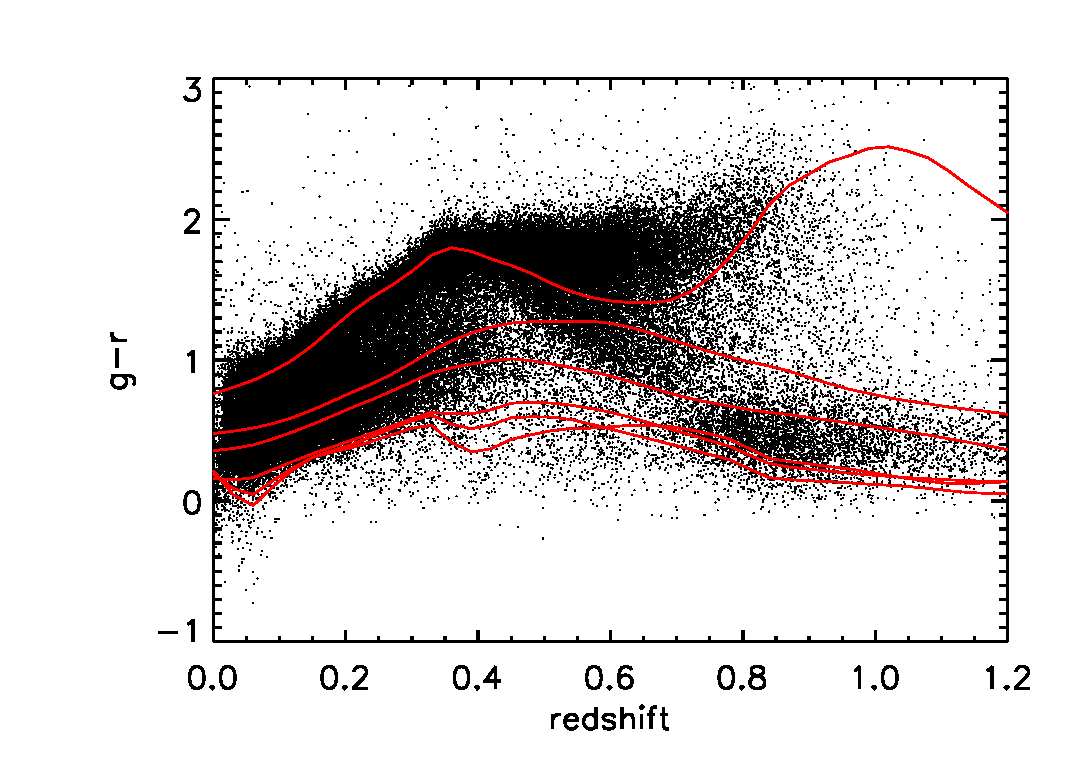
\includegraphics[width=0.5\textwidth]{figures/color_gr_z.eps}
	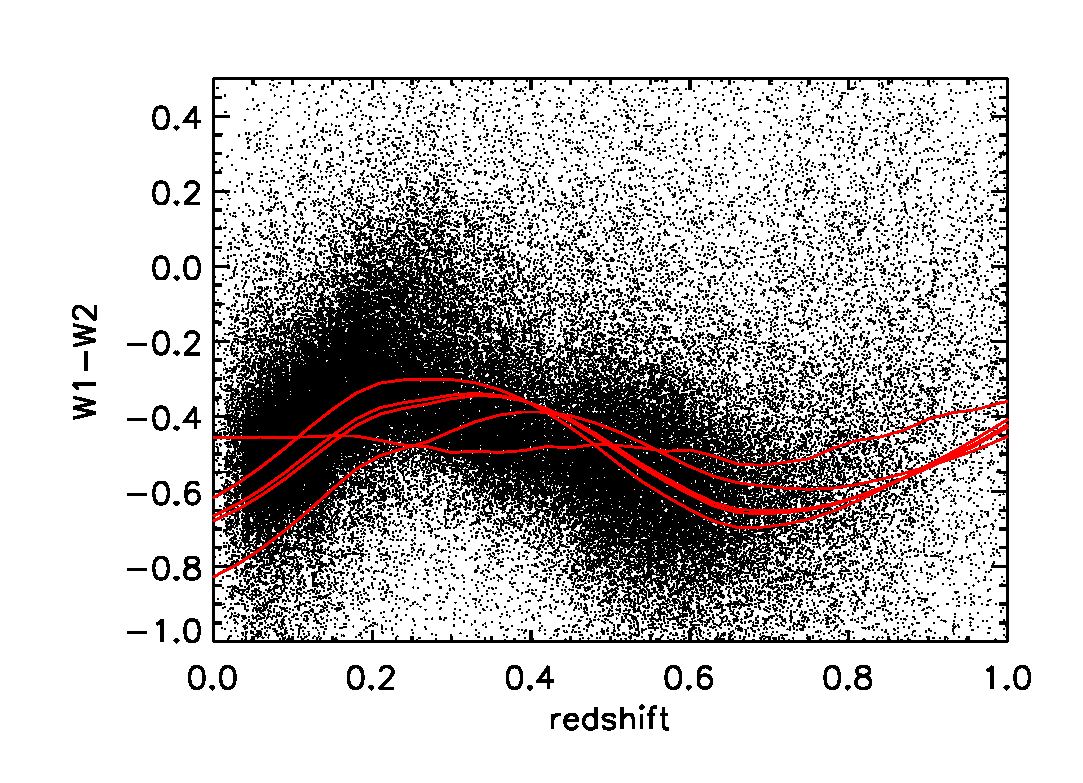
\includegraphics[width=0.5\textwidth]{figures/color_w1w2_z.eps}
	\caption{Color vs. spectroscopic redshift for the whole set of the photometric catalog sources (colored black) with available spectra. Colors of the six CWW+KIN templates as a function of redshift templates are plotted as red lines. These templates alone cover sufficient area on the plane and their linear combination returns reliable photometric redshift.}
	\label{fig:color_z}
\end{figure*}

We list the detailed parameter files that we used in our EAZY run.

\subsubsection{Redshift probability distribution} \label{pdz}

%SED fitting method suffers from the color-redshift degeneracy - redshift probability may have several peaks at significantly different values. One such example could be relatively featureless blue SED that can be fit well at z$\sim$0 and z$\sim$3 as templates can not distinguish between Lyman or Balmer breaks. Ideally one would want to include more bands to break this degeneracy, but as this is usually not possible, EAZY follows \citet[][]{Benitez2000} and uses statistical approach to constrain photometric estimates. Bayesian prior is used to assign different probabilities to different redshifts for a given source with apparent magnitude \textit{m}: low probability is assigned to low redshift due to smaller volume and high redshift due to the lower probability to find extremely bright galaxies. Ideally, redsift distribution should be determined from observed data, but observed samples are generally small and incomplete at high redshifts and for faint sources, so we use prior probability distribution derived with synthetic photometry of the semi-analytic model lightcone catalog described in \S 2.2 in \citet[][]{Brammer2008} and implemented in EAZY.

One is the redshift probability distribution prior. Due to the color-redshift degeneracy, it is not unusual that an SED fit by any $z_{ph}$ tool could have multiple, widely separated peaks in its redshift probability distribution function (PDF), which would then create difficulty in assigining the most probable $z_{ph}$. Following \citet[][]{Benitez2000}, EAZY deals with this problem by using a Bayesian prior of redshift probability distribution in the magnitude domain, $P(z|m)$, which essentially means that an object of magnitude $m$ is unlikely to reside at a redshift that is too lower or too higher than $z$ \citep[see \S 2.2 of][]{Brammer2008}. We adopted the default prior used by EAZY, which is a function of $R$-band magnitude, and treated $r$ as $R$.

\begin{figure}
\begin{minipage}{\columnwidth}
\includegraphics[width=\columnwidth,height=0.28\textheight]{figures/redshift_prior_18_25.png}
\caption{R-band redshift probability distribution prior used in this work for a range of magnitudes from AB 18 (blue) to AB 25 (black) with a step of 1 magnitude.}
\label{fig:redshift_prior}
\end{minipage}
\end{figure}

\subsubsection{Magnitude zeropoint offset}

%The largest advantage of the template fitting method is that derived photometric redshifts can be compared against the full spectroscopic sample. If any systematic offset is present, then it is possible to calibrate either the template library or the input magnitudes. As one of the output EAZY produces observed magnitudes - flux from the best fit template is convolved with the input filter response curve. In all bands we find the non-zero mean difference between input and fitted magnitudes for the sources whose photometric redshift was within 1$\sigma$ from the spectroscopic one.

%\textit{I can add plot "mag\_diff vs $ z_{spec} $" or just a histogram of mag\_diff}

%While generally such offsets in different bands can be redshift- and/or magnitude-dependent, we choose to take it as a constant and apply it to the whole input catalog. The offsets of the AB mag XX, XX, XX, XX, XX, XX, XX for $u'g'r'i'z'W1W2$, respectively are supplied to EAZY and do not modify our original catalog. 

%Application of the magnitude offset reduces standard deviation of the subsample of the galaxies with spectroscopic redshifts from 0.XX to 0.XX (here and below we use the term "standard deviation" for the function $\Delta z/(1+z)$ for the subsample of the galaxies for which 0 $<$ $ z_{ph} $ and 0 $<$ $ z_{spec} $ $<$ 1.5). (p32 of 1008.0395.pdf)

The second is the magnitude zeropoint offset. The synthetic magnitudes ($m_{syn}$) from the best-fit template can never exactly match the input magnitudes ($m$), and this should not be a concern if the statistics shows that the difference ($m_{syn} - m$) in a particular band is random. However, sometimes such a difference shows a systematic offset, which can be caused by a number of reasons, such as a systematic deviation of the templates with respect to the true SEDs, a slight error in the adopted system response curve, etc. To obtain the best results, one could manually correct this systematic difference by applying a zeropoint offset to the input magnitudes. Based on our test using the spectroscopic subset, we found that the offsets are -0.0749, 0.0193, 0.0019, 0.0074, -0.0351, 0.1574, 0.1460 AB in u, g, r, i, z, W1, and W2, respectively, for the EAZY run with all 7 bands and -0.0604, 0.0141, -0.0047, 0.0150, -0.0141 AB in u, g, r, i, z, respectively, for the EAZY run with only 5 SDSS bands. EAZY has the mechanism to apply such offsets, which we used in the fitting process. Our source catalogs, however, are not modified.

%\subsubsection{Outliers in z-W1 }

%We noticed a small fraction of sources bright in z-band, but very dim in W1/W2 that were assigned with $z_{ph}~0$ in every EAZY test while their $z_{spec}$ typically ranged from $0 < z < 0.4$. Visual inspection showed that though some of the sources were intrinsically dim in the near-IR, majority suffers from under-subtraction in T-PHOT and thus their assigned fluxes in W1/W2 are wrong. We selected such sources using criteria z-W1<-1.0 and z<19.9 and assigned them with flux -150 in W1/W2 thus excluding these bands from the template fitting with EAZY.

%data and numbers in script3_eazy_in_outliers_neg150

\subsubsection{EAZY with and without unWISE bands}

%While it is generally accepted that near-IR bands YJHK improve photometric redshift estimation, especially beyond z$\sim$1.3, where the 4000$\AA$ break goes out of the z band and the Lyman break is not yet detectable in the u band, using WISE bands may not be so efficient for two reasons: very few templates extend their models to 3-5$\mu$m and errors associated with the W1 and W2 photometry are much larger than that of the optical bands, hence not giving strict constraints on the choice of the template. Nevertheless, our tests reveal that using W1 and W2 bands moderately improves photometry as compared to using only optical bands ($\sigma=XX$ and $\sigma=YY$, respectively). 

The third point is about incorporating the W1/W2 photometry. For the EAZY runs, we did not find any significant offset of $z_{ph}$ between the one including W1/W2 photometry and the one without (results from both EAZY runs are shown on Fig. \ref{fig:eazy_photo_spec}. Left (right) panel shows $z_{ph}\ vs\ z_{spec}$ for the EAZY run with (without W1/W2 bands). However, based on the spectroscopic subset, inclusion of W1/W2 photometry did improve the $z_{ph}$ quality by reducing the standard deviation of $\Delta z/(1+z_{spec})$ from 0.0296 to 0.0287 and reducing the number of outliers by 837 - from 8,099 to 7,262. Therefore, incorporating W1/W2 photometry is justified. In the catalog we opt to present both flavors of $z_{ph}$ derived by EAZY - using all 7 bands and using only optical SDSS bands (denoted by the index $\it{nowise}$), but in the following discussion we only use 7 band catalog  when refer to EAZY $z_{ph}$.

\begin{figure*}[!ht]
\includegraphics[width=0.5\linewidth]{figures/eazy_spec1.png}
\includegraphics[width=0.5\linewidth]{figures/eazy_nowise_spec.png}
\caption{$z_{ph}$ vs $z_{spec}$ for the subsampe of sources with spectroscopic redshifts from the training sample. Left panel shows results for all 7 bands used in EAZY run and right panel - with only SDSS bands. Black crosses with $z_{ph}\sim 0$ are sources with erroneous fluxes in W1/W2. They are refitted by EAZY using only optical fluxes (see Fig.\ref{fig:zw1}). Black line shows 1:1 relation. }
\label{fig:eazy_photo_spec}
\end{figure*}

%As was mentioned above, only 39\% and 44\% of sources have W1 and W2 photometry, respectively, hence, there is some inconsistency in the input data for the photometric redshift estimation. In addition to that there is a population of sources with z-W1 $>$ XX and W1 - W2 $>$ XX for which photometric redshift is always underestimated. After visual inspection we confirm that though some of them are intrinsically very red sources, majority of them are associated with the bad flux subtraction made by T-PHOT. Those sources were assigned with the magnitude of -95.0 in W1 and W2. For these two reasons we present two photometric redshifts in the catalog - with and without unWISE W1 and W2 bands. Besides the number of the input filters, the rest of the parameters are identical:

The inclusion of W1/W2 photometry does come with a price. Inspecting the results based on the spectroscopic subset, we found a small population of sources with $z-W1<-1.0$ mag and $z<19.9$ mag (Fig.\ref{fig:zw1} left panel). We also found that the vast majority of such sources in the spectroscopic subset always had wrong $z_{ph} \approx 0$ (Fig.\ref{fig:zw1} right panel, green dots). After visually inspect the T-PHOT residual images, we concluded that these extreme colors are predominantly caused by the erroneous T-PHOT results (oversubtraction of the morphological templates). Therefore, we isolate such objects (143,810 or 1\% of the catalog) and derive their $z_{ph}$ without W1/W2 photometry, which improved the quality of the fit (Fig.\ref{fig:zw1} right panel, blue dots).

\begin{figure*}[!ht]
\includegraphics[width=0.5\linewidth]{figures/zw1_outl_color1.png}
\includegraphics[width=0.5\linewidth]{figures/zw1_outl_photoz_spec_z.png}
\caption{Left: sources with known $z_{spec}$ are plotted on a color-magnitude plane. SED of the sources labeled with black crosses are fitted poorly by EAZY when photometry in W1 and W2 bands is included. In green color we show the region defined as $z-W1<-1.0$ mag and $z<19.9$ mag inside which sources will be fitted to EAZY using only optical fluxes. Right panel shows such poor fit on a $z_{ph} vs z_{spec}$ plane (green) and this fit is improved when sources are fitted only with SDSS bands (blue). Black line shows 1:1 relation.}
\label{fig:zw1}
\end{figure*}

As can be seen on Fig.\ref{fig:eazy_photo_spec} both EAZY (red) and EAZY\_nowise (blue) redshifts are in a good agreement with spectroscopic one up to $z_{spec}\sim 0.85$ where the scatter becomes too large. We fix EAZY to fit photometric redshifts up to $z_{max}=1.0$ and discuss this upper limit in Sec. \ref{z_max} in more details.

%Derived photometric redshifts are published with the associated 1$\sigma$ confidence intervals and redshift quality parameter ``odds'' that represents the fraction of the total probability that redshift lies within z$\pm0.2$ of the $ z_{ph} $ estimate, and is designed to identify sources that have broad and/or multi-modal probability distributions.

%The source is assigned the $ z_{ph} $ = -99 when it has input data in less than 3 bands. Number of such sources is low - 2,946 and 11,101 (update after color-color cut) for the EAZY runs with and without unWISE data, respectively.

%The results from the EAZY run are shown on Fig. \ref{fig:eazy_photo_spec} and are also listed in Table x. In addition to the best-fit $z_{ph}$, it also includes the error estimate and the redshift quality parameter ``odds”, the latter of which is unique to EAZY and represents the fractional probability that the true redshift lies within $z_{ph}\pm0.2$. 

%Comparison of the two sets of $ z_{ph} $ shows similar behavior of the  $\Delta z/(1+z)$ with marginally smaller scatter and more linear trend around z$\approx$0 for the data with seven input bands as compared to the no unWISE data.

\subsection{Running ANNz}

ANNz requires a sample of galaxies with known spectroscopic redshifts as the training set to build an empirical relation between measurable parameters and redshifts. While magnitude, surface brightness, color, size, morphology, etc. can all be used as an input node for ANNz, the most commonly used ones are magnitudes and colors, and these were what we adopted. 

%Photometric redshifts derived by ANNz are only reliable for the range of magnitudes or colors of the training set, so the input values should be chosen based on the rate of the overlap between the training set and the full input catalog. Our catalog is not magnitude limited and contains a large fraction of faint sources in all bands except for the r-band, which is used as a base of our catalog. Thus the training set inevitably covers only part of the plane taken by the full catalog, no matter what input values to choose. We randomly divided a sample with spectroscopic redshifts into three subsamples - to train ANNz, validate relations and test the output redshift and performed a set of tests to find the best input node. We tried all seven magnitudes, only optical magnitudes, seven non-redundant colors, combination of seven magnitudes and seven colors, seven magnitudes and three optical colors (except for the u-r) and seven colors with gri magnitudes. We found that seven magnitudes gives the best result and use it as the input node.

Quality of the set of sources used for training, validation and testing defines the perfromance of ANNz. Out of 150,767 sources from the spectroscopic sample we chose 148,567 with the redshift within $0 < z_{spec} < 1.5$ (number density of the sources drops sharply after $z_{spec} < 1.5$ and our set of bands cannot prevent the degeneracy in the redshift determination) and call such subset an ANNz spectroscopic sample. While auxiliary deep surveys (6df, DEEP2, WiggleZ,VIPERS and VVDS) compose only 19.5\% of the total, they are constitute an key portion of the ANNz spectroscopic sample by providing important information about the faint (and thus presumably high-redshift) sources and also filling in the magnitude space in different regions than SDSS spectroscopic sample thus helping to more efficiently train ANNz.

Following the instructions of ANNz, we randomly divided this ANNz spectroscopic sample into three sets of roughly equal number of objects, namely, the training set to train ANNz on our data, the validation set to validate the $z_{ph}$ derivation, and the testing set to find the best choice of the input nodes. We tried following options: all seven magnitudes, only optical magnitudes, seven non-redundant colors, combination of seven magnitudes and seven colors, seven magnitudes and three optical colors (except for the $u-r$) and seven colors with $gri$ magnitudes. After extensive testing, we found that seven magnitudes gives the best result and use it as the input node.

Architecture of the ANNz network can be described as $N_{input} : N_{1} : N_{2} : . . . : N_{m} : N_{output}$, where $N_{input}=7$ is the number of input magnitudes for each object in our sample, $N_{1}, N_{2},. . .$, and $N_{m}$ are the number of nodes in each ANNz hidden layer for a total of $m$ layers, and $N_{output}$ is the number of sets for output photometric redshift, usually set to be 1. We again randomly divided the spectroscopic catalog into three subsamples and tested ANNz for the best combination of the nodes, the hidden layers and the number of iterations. We found that two layers with seven nodes in each layer (7:10:10:1 architecture) with 700 iterations would perform the best with our data.

Depending on the particular seed for the random number generator, the number of iterations and the fraction of the spectroscopic sample used for the weights, the training process usually converges to different redshift local minima. However, it is not necessary to select one best network - in fact, ANNz can use the sub-optimal networks to improve overall accuracy: the mean of the individual outputs from a group of networks usually gives a better estimate for the photometric redshift than the outputs of any network alone. In order to get the full advantage of this feature and also to get a comprehensive validation of the ANNz performance (ANNz performance should only be tested on a subsamples that is not used for either training or validation) we used the following strategy to train ANNz:\\
1. ANNz spectroscopic sample was shuffled in a random order\\
2. The catalog was divided into 3 sets: training set (70\% of sources), validation set (10\%) and testing set (20\%).\\
3. With this set of data ANNz was trained 2 times using different seed for the random number generator and 2 weights files .wts are created.\\
4. Steps 2. and 3. were repeated 4 more times in such a way that each of the five testing sets uses different part of the ANNz spectroscopic sample and thus the whole sample can be independently tested.\\
5. ANNz was ran with 10 weight files on an ANNz spectroscopic sample and then 2,091 outliers identified as sources with $\dfrac{\mid\Delta z \mid }{1+z_{spec}}<0.15$ were rejected.\\
6. Steps 2-4 were repeated for the ANNz spectroscopic sample without outliers and ANNz was ran with 10 new weight files on our Stripe 82 photometric catalog. 

The performance of ANNz must be tested on a subset of sources that has not been used for the training, therefore it is not straightforward to test the quality of $z_{ph}$ for the whole subsample of spectroscopic sources. In our approach the sample of sources with known $z_{spec}$ is divided 5 times into training, validation and test subsets in such a way that 5 test subsets comprise a full ANNz spectroscopic sample. Then we run ANNz on each of these 5 test sets using two weight files per set that were derived using sources from the corresponding training and validation sets. In the end we have a full set of ANNz spectroscopic sample tested by ANNz in a correct way that is plotted on Fig.\ref{fig:annz_highz}. Standard deviation of the sources within $\dfrac{\mid\Delta z \mid }{1+z_{spec}}<0.15$ (i.e. not outliers) is 0.0241 - better than for any EAZY run. 

\begin{figure}
\begin{minipage}{\columnwidth}
\includegraphics[width=\columnwidth,height=0.28\textheight]{figures/annz_highz_photoz_specz_test1.png}
\caption{ANNz $z_{ph}$ vs $z_{spec}$ for the subsampe of sources with spectroscopic redshifts from the training sample. Standard deviation of the sources that are not outliers is 0.0241. Black line shows 1:1 relation.}
\label{fig:annz_highz}
\end{minipage}
\end{figure}

The only difference with the science run of ANNz is that our ANNz spectroscopic sample was tested using 2 corresponding weight files per set, while for the photometric catalog we used all 10 available .wts files, so reported standard deviation should be treated as the upper limit and expected the performance of ANNz on a full set of data is expected to be better than that.

%We chose to present two flavors of photometric redshifts - one derived using the training set with only sources with SDSS $ z_{spec} $ (spec\_SDSS\_only) and the other using the training that incorporates other deeper spectroscopic surveys as well: 6dF, WiggleZ, DEEP2, VVDS and VIPERS (spec\_FULL). While these deeper surveys compose only 19.5\% of the total, they provide important information about the faint (and thus presumably high-redshift) sources and also fill in the magnitude space in different regions than SDSS spectroscopic sample thus helping to more efficiently train ANNz.

%\subsection{Photometric Redshift Errors}

%Errors associated with the photometric redshifts derived with EAZY and ANNz are different: EAZY (and any template fitting code) takes associated flux errors in each band as a region through which a fitted template may go. Larger errors mean more flexibility with the choice of the proper template and does not necessarily leads to the degraded quality of photometric redshift. In such a case two sources with identical input fluxes but different associated flux errors may have different photometric redshift.
%Machine learning on the other hand does not work with the input values as a physical parameters and only sees the relation between it and training set. Thus two sources with similar input magnitudes but different associated magnitude errors will have identical photometric redshift assigned by ANNz, but their photometric redshift errors will be different and proportional to the input magnitude errors.

\subsubsection{Beyond the training set}

\begin{figure*}[!ht]
\includegraphics[width=0.5\linewidth]{figures/color_color_annz_nobulk.png}
\includegraphics[width=0.5\linewidth]{figures/zphot_zspec_annz_nobulk.png}
\caption{Left: Color-color plane of all extragalactic sources with $S/N>5$ in bands $gri$ (blue), training set for ANNz (green) and the subsample of the sources from the training set that poorly cover the color-color plane (red). Right: $z_{ph}$ vs $z_{spec}$ for the subsample of 639 sources from the ANNz spectroscopic sample that poorly cover the color-color plane. Red dots - sources within $\dfrac{\Delta z}{1+z_{spec}}<0.15$ with standard deviation 0.0353, and red crosses - outliers.}
%\hfill
\label{fig:nobulk}
\end{figure*}

A limitation of machine learning is that the results are reliable only when the training set covers the full parameter space of the input nodes. Our spectroscopic sample only covers the brighter part of the catalog, and therefore only covers part of the parameter space of the full catalog, regardless of what input values we use. It is impossible to estimate the performance of ANNz in the regions that are completely uncovered by the training set, but it is important to understand what it would be in the regions that are still populated by the sources from the training set, though sparsely. 
%On a color-color plane on Fig.\ref{fig:nobulk} we plot all sources with $S/N>5$ in bands $gri$ (blue) that have enough sources in the training sample (green) and also sources with $S/N>5$ in bands $gri$ (cyan) that have very few sources from the training sample to determine their $z_{ph}$ (red). Out of 10,403,778 sources only 481,293 fall into this category of being potentially undertrained, and it is important to estimate the performance of ANNz in this region.

For this purpose, we carry out a test by projecting our color space onto the $g-r$ versus $i-z$ color plane, which is shown in the left panel of Fig. 7. We plot all the sources whose $z_{ph}$ are to be derived (i.e., those with $S/N\geq 5$ in the {\it gri} bands) as the cyan dots, and roughly divide the region that they occupy into four parts according to the density of the objects from the spectroscopic sample: densely populated, intermediatly populated, sparsely populated, and not-populated. To outline these regions, the objects from the spectroscopic sample in the first three regions are shown in green, blue, and red, respectively. We test the ANNz performance in the sparsely populated region (red), which includes 481,293 cyan points out of the total of 10,403,778. There are 639 $z_{spec}$ in this region (the red dots in the left panel of Fig. 7), and we compare them to the corresponding ANNz $z_{ph}$ values in the right panel of Fig. 7. Only 75 sources are outliers based on our criterion of $\Delta z/(1+z_{spec}) > 0.15$, which are shown as the red crosses. The rms value for the rest is 0.0353. For comparison, the rms value for the full ANNz test is 0.0241 after discarding the outliers  (see \S xxx above). Therefore, the ANNz performance in the sparsely populated region is still reasonable. 

While we cannot evaluate the performance in the ``not populated’’ region, we conclude that this is not a serious concern because the objects in this region are of a small fraction of the total. In this particular case, they constitute only 4.6\% of the full catalog. The vast majority of them are faint sources, most of which have high $z_{ph}$ and do not enter the final $z_{ph}$ catalog because of the redshift limit that we impose to this catalog (see \S 5.3 below).

%We test ANNz performance on a subset of 639 sources (red dots from the left panel of Fig.\ref{fig:nobulk}) from the ANNz spectroscopic sample that sparsely populate the color-color plane of the full photometric catalog. Only 75 sources are outliers (using a standard definition $\dfrac{\Delta z}{1+z_{spec}}>0.15$) and are denoted with red crosses on the right panel of Fig.\ref{fig:nobulk}; and standard deviation of the rest of the subsample is 0.0353. Our conclusion is that though standard deviation is obviously higher than that for the bulk of the sources from ANNz (0.0241), but the difference is not very severe and it only affects 4.6\% of the sources (cyan on the left panel of Fig.\ref{fig:nobulk}), most of them are faint and (presumably) high-redshift and thus will likely be discarded from the final catalog (see \S 5.3) and will not significantly degrade the quality of our data.


\section{Discussion}

%In this section derived photometric redshifts are discussed, compared to one another and to other available photometric redshift surveys.

In this section, we further examine our $z_{ph}$, and compare them to other photometric redshift surveys in this field.


\subsection{Cleaning of $z_{ph}$ Catalog}

We derived $z_{ph}$ for all the objects in our extragalactic catalog, however some objects should not be included in the final $z_{ph}$ catalog for obvious reasons.
For the objects that have photometry in less than three bands, their EAZY $z_{ph}$ are deemed to be unreliable and are assigned $z_{ph}=-99$. There are only 2,946 (11,101) such objects when W1/W2 are (not) included.

%ANNz computes the photometric redshift based on the training sets without "knowing" the physical nature of both input and output information. This means that if a source under question does not lay close to the sources from the training set in a space of input parameters (i.e. 7 input magnitudes), ANNz calculates photometric redshift by extrapolating the known relations. As a result 163 sources have negative redhifts ranging from $-0.116 < z_{ph} < 0$. We determine 27 sources with known $z_{spec}$ that ranges from 0 to 0.045 and standard deviation of the redshift difference is only 0.020. Thus though negative redshift is obviously a wrong value, numerically ANNz $z_{ph}$ is within accepted scatter and proves the quality of the ANNZ performance. Nevertheless, all 163 sources are excluded from the following discussion.

Some objects from the ANNz run should also be discarded, but for a different reason. If a source is outside of the region in the input parameter space where the training set populates, the ANNz calculates $z_{ph}$ by extrapolation. As the ANNz does not care about the physical meaning of any input or output parameters, sometimes the extrapolation could result in negative $z_{ph}$. There are 163 such objects with $z_{ph}$, and as it turns out, 27 of them have $z_{spec}$, which range from 0 to 0.045 while their $z_{ph}$ goes from -0.014 to 0. The maximum photometric redshift error for these 27 sources is 0.085, mean photometric redshift error is 0.0374 and standard deviation is only 0.0215 - well below the value for the full photometric catalog.

%We want to remind that the catalog is based on the r-band detection with SNR $>$5 and contains a lot of sources barely detected or undetected at all in the other bands. Nevertheless both EAZY and ANNz would still provide such objects with a photometric redshift, though potentially unreliable. We select 10,403,778 sources (72\% of the total extragalactic catalog) with S/N $>$ 5 in $gri$ bands and use this subsample in the following discussion.

As our photometric catalog is based on the r-band detections with $S/N\geq 5$, it contains many sources that are weaker or even invisible in other bands and their $z_{ph}$ could be unreliable. Therefore, we only focus on the objects that have $S/N\geq 5$ in at least the {\it gri} bands. There are 10,403,778 sources that meet this requirement, which constitute 72\% of the total extragalactic catalog. Our discussion below will be based on this subsample.

\subsection{Comparison between ANNz and EAZY photometric redshifts}

In this section we compare $z_{ph}$ derived with ANNz and EAZY, discuss how do they differ and what could be the reasons for it.

Both algorithms, SED fitting and machine learning, rely their photometric redshift estimation on a detection of characteristic features in a galaxy spectrum. Observed wavelength of this characteristic feature unambiguously defines the redshift of a source under question. Such features usually manifest themselves as a sharp drop in magnitudes - Ly limit, $Ly\ \alpha$ break, PAH features, etc. For our range of bands and expected range in the redshifts such a feature is a $4000\AA$/Balmer break that is caused by the absorption by hydrogen atoms of photons with energy above the Balmer limit (3,646$\AA$) and also by the combination of the absorption features by ionized metals in the stellar atmospheres.

Because of the absence of other prominent features, relative location of a $4000\AA$/Balmer break explains almost every non-linear behavior of the $z_{ph}$ vs $z_{spec}$. 

At $z\sim 0$ this break falls into the $u$ band, one of the two most shallow SDSS bands, and causes the kink in the range $0 < z < 0.1$. This kink is the most prominent in the EAZY\_nowise sample, in which no information from the near-IR bands can be used to break this degeneracy. As local galaxies are not usually bright in the near-IR, ANNz machine learning algorithms also do not get much information that can be used to refine the fit. Surprisingly, adding W1/W2 bands to the EAZY helps to improve the fit - though CWW+KIN templates that we adopt here do not contain any near-IR features, steady decrease in the relative flux from $\sim 1.2 \mu$ in all templates helps to constrain the $z_{ph}$ even in the case of no detection (what is exactly expected for the sources at $z\sim 0$).

A well-known scatter around $z\sim0.4$ is caused by the $4000\AA$/Balmer break that falls in the dip between $g$ and $r$ bands - the construction of the instrument is such that this dip is the largest among all four dips in the optical.

%\subsubsection{Maximum $z_{ph}$} \label{z_max}

This break also defines the upper limit of the EAZY $z_{ph}$ - at $z\sim 0.9$ it falls between $i$ band and $z$ band which is the most shallow among SDSS, and the scatter of the $z_{ph}-z_{spec}$ immediately increases. But also the SDSS depth starts to become important as the $S/N$ ratio of high-z sources gets much worse. 

This scatter is however not due to $z_{max}$ that we assigned to EAZY, which sets the upper limit to the allowed photometric redshift - we tested larger values to confirm that it does not put high-z galaxies closer to the true $z_{ph}$, but on contrary - it assigns low-z galaxies with unrealistic $z_{ph}\sim 1$ thus increasing the overall scatter. Thus our choice of $z_{max}=1$ as a reasonable limit for the EAZY is justified.

While ANNz behaves considerably better in this redshift range and (due to the inclusion of the deep surveys from the ANNz spectroscopic training sample) have a much tighter $z_{ph}$ vs $z_{spec}$ relation as compared to the EAZY, at $z_{spec}\sim 1.1$ machine learning algorithm starts to fail and underpredicts $z_{ph}$ (Fig.\ref{fig:annz_highz}) - result of the low number of the galaxies in the training set and an overall decrease of the $S/N$ in all 7 input nodes. 

%\subsubsection{Redshift distribution}

\subsection{Contamination with high-z sources} \label{high-z}

Considering similar behavior on the $z_{ph}$ vs $z_{spec}$ plots one could expect also the similar shape of the redshift distribution for all three flavors of derived $z_{ph}$ for the full sample. But as one may see on Fig. \ref{fig:hist_3zphot}, these distributions are very different - both EAZY $z_{ph}$ have a sharp single peak around $z\sim 0.4$ and a steady decrease in the number density up to the assigned $z_{max} = 1$, while ANNz produces a double peak distribution with the first one at a similar redshift as the EAZY one and the second, even larger peak being at $z\sim 0.9$. While this second peak is not fully nonphysical - we estimated stellar masses in the equal comoving volume bins of $20\ Mpc^3$ and verified that there is no stellar mass decrease - this drastic difference requires explanation. We anticipate that both algorithms and all 3 flavors of $z_{ph}$ produce similar results \textit{in the redshift range of our interest, i.e. $0 < z < 0.85$} and behaves differently at higher redshifts.

\begin{figure}
\begin{minipage}{\columnwidth}
\includegraphics[width=\columnwidth,height=0.28\textheight]{figures/hist_3zphot.png}
\caption{Photometric redshift distribution. Red - EAZY, blue - EAZY\_nowise, green - ANNz.}
%\hfill
\label{fig:hist_3zphot}
\end{minipage}
\end{figure}

Stacked Stripe 82 images should contain a lot of high-z sources in contrast to the single-epoch SDSS data. We tested this hypothesis by comparing the number of low- and high-z sources that would be detected in a stacked Stripe 82 image and in a single-epoch SDSS image, using CFHTLS data. Subsampes were constructed in the following way: the galaxy (StarGal=0) that has $S/N>5$ in $gri$ bands, and $0<phot\_z <9$ is visible in Stripe 82 (SDSS) if it is $r<24.8\ (22.7)$ AB. It is a low-z sources if $photo\_z\leq0.834$ and a high-z source if $photo\_z>0.834$. We chose $z=0.834$ as this is the redshift of an edge of a sphere with comoving volume of 100 $Mpc^3$ that will shall bin into 20 $Mpc^3$ slices to study evolution of the galaxy population.

Fig.\ref{fig:hist_lowz_highz} shows a redshift distributions for the low-z Stripe 82 (blue), SDSS (grey) and for the high-z Stripe82 (green) and SDSS (magenta) sources. Vertical red lines defines our choice of separating high-z from the low-z sources. The drop in the number of sources is very sharp for SDSS - there are 11.5 times more low-z sources as compared to the high-z ones (1,434,791 vs. 124,905). The situation with the Stripe82 sources is quite different - there are only 1.4 times more low-z sources as compared to the high-z ones (3,684,728 vs. 2,629,236).

One more hint on a large fraction of the high-z sources in our data comes from the fact that 32.4\% of the high-z sources from the spectroscopic sample are cross-matched with our photometric catalog with the matching radius of 2''.
For the set of filter used in this project both EAZY and ANNz cannot treat high-z sources properly and assign them correct redshift, therefore such sources should be removed from the catalog. Due to the high fraction of faint sources that populate large area on a color-color plane, such high-z sources cannot be removed based on their colors.

\begin{figure}
\begin{minipage}{\columnwidth}
\includegraphics[width=\columnwidth,height=0.28\textheight]{figures/hist_lowz_highz_CFHTLS.png}
\caption{Histogram shows the redshift distribution of the CFHTLS data for the low-z (blue) and high-z (green) sources detected in Stripe82 images as compared to the low-z (grey) and high-z (magenta) sources in SDSS single-epoch images. Red vertical line at z=0.834 separates low-z from high-z galaxies. Stacked images are $\sim2$ magnitudes deeper and contain a lot of high-redshift sources that contaminate our sample and should be removed from the catalog}
\label{fig:hist_lowz_highz}
\end{minipage}
\end{figure}

We propose to remove high-z fraction from our sample using the difference in the treatment of such sources by EAZY and ANNz - as we discussed above, while EAZY scatters high-z sources all over the allowed redshift range (this is fortified by the use of the redshift probability distribution introduced in Sec.\ref{pdz}), while ANNz tends to assign such high-z sources with the maximum redshift for which it has sufficient number of galaxies from the training set ($z\sim 1.1$. On a Fig.\ref{fig:criteria} we plot EAZY $z_{ph}$ - ANNz $z_{ph}$ and draw a horizontal line at -0.4 - sources that fall below this line are considered as high-z with bad fit and are rejected from the catalog. This further reduces the number of sources in the catalog to 8,214,318 (blue dots on Fig. \ref{fig:criteria}) and rejects 2,189,460 (green dots). Majority of the rejected sources are high-z sources and fall beyond our redshift of interest (denoted with the red vertical line).

\begin{figure}
\begin{minipage}{\columnwidth}
\includegraphics[width=\columnwidth,height=0.28\textheight]{figures/high_z/criteria.png}
\caption{Difference of the $z_{ph}$ produced by EAZY and ANNz is used as a criteria for rejection of the high-z sources. Blue points lay above $EAZY\ z_{ph}\ -\ ANNz\ z_{ph} = -0.4$ show similar behavior with both codes and are left in the catalog, while green dots - the one that lay below the black line are rejected - most of them are high-z sources that are poorly fitted by either EAZY, ANNz or both algorithms. Red line at z=0.834 defines the redshift limit of our interest - our catalog is neither secure in terms of photometric redshift estimation, nor complete even at $M_{\ast}$.}
\label{fig:criteria}
\end{minipage}
\end{figure}

\
{\it I rewrote till this phrase}

\

-Different photoz flavours treat these high-z source differently:
	EAZY full and EAZY\_nowise distribute them more or less homogeneously with a peak at $\sim0.75$ while ANNz puts all of the high-z sources at $z\sim0.89$ and this is a good way of removing them!
	
This behavior is significantly different to the EAZY one, that just scatters high-z sources all over the $z_{ph}\ vs\ z_{spec}$ plane - we shall use this in the \S \ref{high-z} when attempt to remove high-redshift sources from our sample.	
	
\begin{figure}
\begin{minipage}{\columnwidth}
\includegraphics[width=\columnwidth,height=0.28\textheight]{figures/hist_highz.png}
\caption{OLD DATA! Photometric redshift distribution of the sources with $z_{spec}>1$. Red - EAZY, blue - EAZY\_nowise, grey - ANNz\_full, green - ANNz\_sdss}. Both photometric redshifts produced by ANNz have sharper peaks and this can be used to eliminate such high redshift sources from our sample.
%Right panel: histogram of the mean ratio of the original magnitude errors over magnitude errors in the "g matched to u" image for each of 5,556 images. Black vertical line denotes the mean ratio of 1.}
%\hfill
\label{fig:hist_highz}
\end{minipage}
\end{figure}

Reference to the subsection: \S \ref{high-z}

\subsection{Comparison with existing photometric redshifts}

Testing our results against available surveys with photometric redshifts is not a direct way to test the quality of our results as errors are on both sides, but such surveys has much more sources as compared to the available spectroscopic samples and provide important statistical insights. We compared all three versions of photometric redshifts derived in this project to photometric redshifts in SDSS DR14 (\citet[][]{Beck2016}, photometric redshifts are updated in DR12 and are unchanged in DR13 and DR14, we refer to it as SDSS DR14); redshifts, derived in \citet[][]{Reis2012} (we referred to it as Reis) using artificial neural network technique, redshifts based on imaging data of the SCUSS, SDSS and WISE surveys and presented in \citet[][]{Gao2018} (we refer to it as SCUSS+SDSS+WISE) and Canada-France-Hawaii Telescope Legacy Survey ``Wide'' survey from data release T0007 (referred to as CFHTLS). Several relations between photometric redshifts are plotted on Fig.\ref{fig:photoz}. Table \ref{table:photoz_matched} contains information about number of matched sources and median redshift of the surveys (all sources in supplementary catalogs were matched to sources with S/N $>$ 5 in $gri$ bands using a 2'' matching radius) and Table \ref{tab:photoz_STD} shows standard deviation for all pairs of photometric redshifts.

\begin{table}
    \caption{Matched photometric redshift surveys}
\begin{tabular}{|p{3.3cm}|p{2.4cm}|p{1.3cm}|}    
        \hline
        Survey                 & Number of matched sources & Median redshift    \\
        \hline
        \textbf{SDSS DR15}  & 12 hours & \\
        \textbf{Reis}     & 8,312,976  & 0.749    \\
        \textbf{SCUSS+SDSS+WISE} & 12 hours & \\
        \textbf{CFHTLS}         & infinite &\\
        \hline
    \end{tabular}
    \label{table:photoz_matched}
\end{table}

- we discuss, how this can influence the GSMD estimation.

- redshift bins: 20 Gpc$^3$ using standard cosmology; number of galaxies per bin; last 5th bin is not used in estimation of the GSMD, but to reject all high-z galaxies

- completeness of the catalog - as seen from the distribution, catalogs are incomplete after z=0.45. Thus Stripe 82 does not produce complete catalog at significantly deeper redshifts as was anticipated, but still has much more data at higher redshifts.


\begin{table*}[t]
  \begin{center}
    \caption{Standard deviation of $\dfrac{\Delta z}{1+z}$ for pairs of photometric redshifts.}
    \begin{threeparttable}
    \begin{tabular}{|p{2.0cm}|p{2.0cm}|p{1.5cm}|p{2.0cm}|p{1.5cm}|p{1.5cm}|p{1.5cm}|}
      \toprule % <-- Toprule here
      \textbf{} &  \textbf{EAZY\_nowise} & \textbf{ANNz} & \textbf{SDSS DR14} & \textbf{Reis} & \textbf{SCUSS + SDSS + WISE} & \textbf{CFHTLS} \\
         \hline 
      \textbf{EAZY}  &   0.0667 & 0.1199 & 0.958 & & &\\
      \textbf{EAZY\_nowise}  &    & 0.0953 & 0.0686 & & & \\
      \textbf{ANNz} & &  &0.0697 & & &\\
   \hline 
    \end{tabular}
\begin{tablenotes}    
    \item[$^1$] Spectroscopic sample is limited to $z_{spec}<1$ for EAZY and to $z_{spec}<1.3$ for ANNz.
     \end{tablenotes}
         \label{tab:photoz_STD}
    \end{threeparttable}
  \end{center}
\end{table*}

SCUSS, SDSS DR15, Reis et al, CFHTLS

%inserted from VICS82 survey https://arxiv.org/pdf/1705.05451.pdf : Both fits give residuals consistent with zero, with a scatter that increases significantly beyond z > 0.8. Interestingly, the addition of the VICS82 does not significantly improve the ac- curacy of photometric redshifts compared to the optical photometry alone. A possible reason is that the main features driving the photometric redshift fit (e.g. the 4000Å break) are still in the optical bands at z < 1. At z > 1, where we might expect gains in the photometric redshift fitting when including VICS82 photometry, the SDSS depth starts to become impor- tant in the signal-to-noise ratio of high-z sources. In this case, the VICS82 data should provide a greater improvement on photometric redshifts when matched to DES or the forthcom- ing J-PAS data on Stripe 82.

%phrasing for the zphot vs zspec: The solid black line represents the equality of the two redshift variables.

%\subsection{FAST} 
%	from Conroy review 2013:
	
%	There has been some confusion in the literature regarding the importance of restframe NIR photometry for estimating stellar masses. First, as indicated in Figure 5, for smoothly varying SFHs, photometry at and redward of the V -band is sensitive to the same light- weighted age, and so redder bands do not provide stronger constraints on the mean stellar age. Taylor et al. (2011) analyzed mock galaxies and concluded that the addition of NIR data did not yield more accurate masses. Taylor et al. also found that different SPS models produced good agreement in derived properties when NIR data was excluded from their fits, but poor agreement when NIR was included. These authors also found much larger residuals in their SED fits when NIR data were included, suggesting that the models are still poorly calibrated in this regime. As discussed in Section 5.2, the NIR is at present probably most useful for constraining metallicities (within the context of a particular SPS model), and so NIR data may be useful in cases where there is a degeneracy between M / L and Z. In general however stellar mass estimates do not appear to be strongly improved with the addition of NIR data, at least with currently available models. Exceptions to this rule may be made for galaxies with very high dust opacities.

\begin{figure*}[!ht]
\centering
\includegraphics[width=0.45\linewidth]{figures/photoz/eazy_eazy_nowise.png}
\includegraphics[width=0.45\linewidth]{figures/photoz/annz_eazy.png}
\newline
\includegraphics[width=0.45\linewidth]{figures/photoz/eazy_dr15.png}
\includegraphics[width=0.45\linewidth]{figures/photoz/annz_reis.png}
\newline
\includegraphics[width=0.45\linewidth]{figures/photoz/eazy_nowise_scuss.png}
\includegraphics[width=0.45\linewidth]{figures/photoz/annz_scuss.png}
\newline
\includegraphics[width=0.45\linewidth]{figures/photoz/eazy_cfhtls.png}
\includegraphics[width=0.45\linewidth]{figures/photoz/annz_cfhtls.png}
\newline
\caption{Comparison of 3 different versions of $z_{ph}$ to each other and available surveys with known photometric redshifts: SDSS DR15, Reis, SCUSS and CFHTLS}
%\hfill
\label{fig:photoz}
\end{figure*}

\subsection{Outliers}
Check my notes p8. and section 4.8 of Dahlen et al 2013

Majority of outliers ($ z_{ph} $ - $ z_{spec} $)$/$(1 + $ z_{spec} $)$>$3 $\sigma$ are diiferent for different codes, 1250 of them are outliers in all 4 codes and also outliers in SCUSS, Reis, CFHTLS and SDSS DR15 (which are photo-z catalogs).
460 of them have zWarning=4 from SDSS DR14 (chi-squared of best fit is too close to that of second best), so it is not necessary that our photo-z are wrong. So it is possible that the real fraction of outliers is even smaller than reported here.

%Photometric redshifts are estimated by fitting the broadband photometry of each source in the photometric catalog to a set of different templates. The goodness of fit is verified by comparing derived photometric redshifts to the available spectroscopic data. Three publicly available SED fitting codes, namely HYPERZ \citep{Bolzonella2011}, LePhare \citep{Arnouts2011} and EAZY \citep{Brammer2008}, were tested, and the later showed the smallest standard deviation when compared to the SDSS DR14 spectroscopic redshifts. Color vs. redshift plot on Figure~\ref{fig:color_z} verifies that templates provided by Coleman, Wu $\&$ Weedman (1980) and Kinney et al. (1996) (CWW+KIN) and extended by Arnouts et al. $$(http://www.oamp.fr/people/arnouts/LE_PHARE/)$$ cover the whole plane of our data. Spectroscopic data also constrains the largest redshift, that is available in Stripe 82 - number counts drops significantly after z$\approx$0.9.

%\begin{figure*}[!ht]
%	\includegraphics[width=0.5\textwidth]{figures/photoz_7band.eps}
%	\includegraphics[width=0.5\textwidth]{figures/photoz_nowise.eps}
%	\caption{Photometric redshift vs. spectroscopic redshift. Sources in photometric catalog and SDSS DR14 spectroscopic catalogs are matched using 1$``$ matching radius}
%	\label{fig:photo_z}
%\end{figure*}

\section{Galactic catalog}

That many stars based on CLASS\_STAR in gri and color-color diagram. all have SNR $>$ 5 in r-band.

\section{Summary}

\acknowledgements

\bibliography{ms}{}
%\input{table3_allpar.tex}

\newpage
%\centerline{ {\bf APPENDIX}}
\appendix

\subsection{EAZY parameters}

TEMPLATES\_FILE       CWW\_KIN.spectra.param \# Template definition file\\
TEMPLATE\_COMBOS      a                  \# Template combination option\\
APPLY\_IGM            y                  \# Apply Madau 1995 IGM absorption\\
N\_MIN\_COLORS         3                 \# Require N\_MIN\_COLORS to fit\\
APPLY\_PRIOR          y                  \# Apply apparent magnitude prior\\
PRIOR\_FILE           templates/prior\_K\_extend.dat \# File containing prior grid\\
Z\_MIN                0.01               \# Minimum redshift\\
Z\_MAX                1.0                \# Maximum redshift\\
Z\_STEP               0.005               \# Redshift step size\\
Z\_STEP\_TYPE          1                 \#  0 = Z\_STEP, 1 = Z\_STEP*(1+z)\\
GET\_ZP\_OFFSETS       y                 \# Look for zphot.zeropoint file and compute zeropoint offsets\\

\section{Acknowledgments}
This publication makes use of data products from the Wide-field Infrared Survey Explorer, which is a joint project of the University of California, Los Angeles, and the Jet Propulsion Laboratory/California Institute of Technology, funded by the National Aeronautics and Space Administration. Part of our data processing and analysis were done using the HPC resources at the University of Missouri Bioinformatics Consortium (UMBC).

\end{document}
